% pdflatex -shell-escape software-analysis-main.tex
\documentclass[12pt,openany]{book}

\usepackage{kotex}
\usepackage{enumerate}
\usepackage{commath}
\usepackage{pifont} %http://ctan.org/pkg/pifont

\usepackage{stmaryrd} %llbracket
\usepackage{slantsc}
\usepackage{hyperref}
\usepackage{adjustbox}

\usepackage{array,booktabs}
\usepackage{multirow}
\usepackage{tabularx}


% Packages for formatting
%\usepackage[margin=1in]{geometry}
%\usepackage{fancyhdr}
%\usepackage{graphicx}
%\usepackage{amsmath}
%\usepackage{amsthm}
%%\usepackage{algorithm2e,setspace}
%\usepackage{algpseudocode}
%%\usepackage{xcolor}
%\usepackage{amssymb}
\usepackage{amsthm}

% Define custom theorem styles
\newtheoremstyle{dotless} % Name of the style
{3pt} % Space above
{3pt} % Space below
{\itshape} % Body font
{} % Indent amount
{\bfseries} % Theorem head font
{} % Punctuation after theorem head
{2.5mm} % Space after theorem head
{} % Theorem head spec

\newtheoremstyle{definitionstyle} % Name of the style
{3pt} % Space above
{3pt} % Space below
{} % Body font
{} % Indent amount
{\bfseries} % Theorem head font
{.} % Punctuation after theorem head
{2.5mm} % Space after theorem head
{} % Theorem head spec

% Applying custom styles
%\theoremstyle{dotless}
\newtheorem{theorem}{Theorem} % Theorem environment with section-wise numbering
\newtheorem*{theorem*}{Theorem} % Theorem environment with section-wise numbering
\newtheorem*{lemma*}{Lemma} % Theorem environment with section-wise numbering
\newtheorem*{proposition*}{Proposition} % Theorem environment with section-wise numbering
\newtheorem*{corollary*}{Corollary} % Theorem environment with section-wise numbering
\newtheorem{proposition}[theorem]{Proposition} % Theorem environment with section-wise numbering
\newtheorem{lemma}[theorem]{Lemma} % Lemma shares the counter with theorem
\newtheorem{corollary}[theorem]{Corollary} % Corollary shares the counter with theorem

\theoremstyle{definitionstyle}
\newtheorem*{observation}{\textcolor{magenta}{Observation}}
\newtheorem*{illustration}{\textcolor{teal}{Illustration}}
\newtheorem*{torus}{{\color{red}T}{\color{orange}o}{\color{green!75!black}r}{\color{cyan}u}{\color{violet}s}}
\newtheorem{definition}{Definition} % Definition shares the counter with theorem
\newtheorem{example}{Example} % Example shares the counter with theorem
\newtheorem{exercise}{{Exercise}} % Example shares the counter with theorem
\newtheorem{remark}{Remark} % Remark shares the counter with theorem
\newtheorem*{note}{Note}
\newtheorem*{notation}{Notation}

\newtheorem*{axiom*}{Axiom}
\newtheorem*{definition*}{Definition} % Definition shares the counter with theorem
\newtheorem*{example*}{Example} % Example shares the counter with theorem
\newtheorem*{exercise*}{\textcolor{teal}{Exercise}} % Example shares the counter with theorem
\newtheorem*{remark*}{Remark} % Remark shares the counter with theorem


\input{preambles/layout}
\usepackage{tcolorbox}
\tcbset{colback=white, arc=5pt}

\definecolor{axiomcolor}{HTML}{a88bfa}
\definecolor{defcolor}{RGB}{52, 152, 219}
\definecolor{procolor}{RGB}{241, 196, 15}
\definecolor{thmcolor}{RGB}{231, 76, 60}
\definecolor{lemcolor}{RGB}{155, 89, 182}
\definecolor{corcolor}{RGB}{46, 204, 113}
\definecolor{execolor}{RGB}{90, 128, 127}

% Define a new command for the custom tcolorbox
\newcommand{\axiombox}[2][]{%
	\begin{tcolorbox}[colframe=axiomcolor, title={\color{white}\bfseries #1}]
		#2
	\end{tcolorbox}
}

\newcommand{\defbox}[2][]{%
	\begin{tcolorbox}[colframe=defcolor, title={\color{white}\bfseries #1}]
		#2
	\end{tcolorbox}
}

\newcommand{\probox}[2][]{%
	\begin{tcolorbox}[colframe=procolor, title={\color{white}\bfseries #1}]
		#2
	\end{tcolorbox}
}

\newcommand{\thmbox}[2][]{%
	\begin{tcolorbox}[colframe=thmcolor, title={\color{white}\bfseries #1}]
		#2
	\end{tcolorbox}
}

\newcommand{\lembox}[2][]{%
	\begin{tcolorbox}[colframe=lemcolor, title={\color{white}\bfseries #1}]
		#2
	\end{tcolorbox}
}
\usepackage{tikz}
\usepackage{tikz-cd}
\usetikzlibrary{shadows}
\usetikzlibrary{shapes.geometric, arrows.meta, positioning}
\input{preambles/algorithm}
\input{preambles/listing}
\input{preambles/commands}

\newcommand{\CP}{\mathbb{CP}}
\newcommand{\M}{\mathcal{M}}

\begin{document}
\begin{titlepage}
    \centering
    
    \vspace*{1cm}
    
    \Huge\textsf{\textbf{Notes on Complex Analysis and
    		Riemann Surface Theory toward Algebraic Geometry}}
    
    \vspace{0.5cm}
%    \LARGE\textsf{- A Journey from Concretization to Abstraction -}
    
    \vspace{1.5cm}
    \textbf{Ji, Yonghyeon}

    \vfill
    A document presented for\\
    the Algebraic Geometry
    
    \vspace{0.8cm}
%    {\large\textsf{Department of Cyber Security}\par}
%    {\large\textsf{College of Science and Technology}\par}
%    {\large\textsf{Kookmin University}\par}
    \vspace{.25in}
    {\large \textsf{\today}\par}
    
%    \Large{Institution Name}\\
%    Date
\end{titlepage}


\tableofcontents
\newpage

\chapter{Elliptic Curve and Torus}
\section{Note 1: Meromorphic Function and Order}

\newpage
\section{Note 2: Meromorphic $f\in\C^X$ and Holomorphic $F\in(\CP^1)^X$}
Given a meromorphic $f:X\to\C$ on a Riemann surface $X$, we define \[
\fullfunction{F}{X}{\CP^1}{p}{F(p)=\begin{cases}
[f(p):1] &\text{if $p$ is not a pole} \\
[1:0] &\text{if $p$ is a pole}
\end{cases}}
\]
\begin{figure}[h!]\centering
\includegraphics[scale=1]{tikzs/X_to_CP1}
\end{figure}

\medskip\noindent
In other word, \begin{figure}[h!]\centering
% https://q.uiver.app/#q=WzAsOCxbMCwwLCJYIl0sWzIsMCwiXFxtYXRoYmJ7Q30iXSxbNCwwLCJcXG1hdGhiYntDUH1eMSJdLFswLDEsInBfe1xcdGV4dHtub24tcG9sZX19Il0sWzAsMiwicV97XFx0ZXh0e3BvbGV9fSJdLFsyLDEsImYocCkiXSxbNCwxLCJbZihwKToxXSJdLFs0LDIsIlsxOjBdIl0sWzAsMSwiZiJdLFsxLDIsImkiXSxbMyw1LCIiLDAseyJzdHlsZSI6eyJ0YWlsIjp7Im5hbWUiOiJtYXBzIHRvIn19fV0sWzUsNiwiIiwwLHsic3R5bGUiOnsidGFpbCI6eyJuYW1lIjoibWFwcyB0byJ9fX1dLFs0LDcsIiIsMCx7InN0eWxlIjp7InRhaWwiOnsibmFtZSI6Im1hcHMgdG8ifX19XV0=
\[\begin{tikzcd}
	X && {\mathbb{C}} && {\mathbb{CP}^1} \\
	{p_{\text{non-pole}}} && {f(p)} && {[f(p)\;\text{:}\;1]} \\
	{q_{\text{pole}}} &&&& {[1\;\text{:}\;0]}
	\arrow["f", from=1-1, to=1-3]
	\arrow["i", from=1-3, to=1-5]
	\arrow[maps to, from=2-1, to=2-3]
	\arrow[maps to, from=2-3, to=2-5]
	\arrow[maps to, from=3-1, to=3-5]
\end{tikzcd}\]
\end{figure}

\newpage
% Examples: meromorphic f and holomorphic F:X->CP^1
\subsection{Example 1: \(X = \mathbb{CP}^1\) (Riemann sphere)}
We view \(\mathbb{CP}^1\) as the Riemann sphere. On the affine chart \[
U_1 = \{[z_0:z_1]\in\mathbb{CP}^1 \mid z_1\neq 0\},
\] we use the coordinate $z = {z_0}/{z_1}.$ The point at infinity is \(\infty = [1:0]\).

On \(\mathbb{CP}^1\), a meromorphic function is the same as a rational function.
Take for instance
\[
f(z) = \frac{z^2 - 1}{z - 2}.
\]
This is meromorphic on \(\mathbb{CP}^1\), with a simple pole at \(z=2\), and (possibly) a pole at \(\infty\).

Define
\[
F:\mathbb{CP}^1\to\mathbb{CP}^1,\qquad
F(p) =
\begin{cases}
	[f(p):1], & p \text{ not a pole of } f,\\[4pt]
	[1:0], & p \text{ a pole of } f.
\end{cases}
\]

Concretely, for \(p=[z:1]\) with \(z\neq 2\),
\[
F([z:1]) = [f(z):1] = \left[\dfrac{z^2-1}{z-2}:1\right],
\]
and at the pole \(p=[2:1]\),
\[
F([2:1]) = [1:0].
\]
Similarly one checks the value at \(\infty=[1:0]\) using the behavior of \(f(z)\) as
\(|z|\to\infty\).

To see that \(F\) is holomorphic, we use the usual charts on \(\mathbb{CP}^1\):

\begin{itemize}
	\item \textbf{At a non-pole point \(p\).} Suppose \(p\) is not a pole of \(f\).
	Then \(f\) is holomorphic near \(p\) and finite there, so \(F(p)=[f(p):1]\in U_1\).
	Let
	\[
	w = \frac{z_0}{z_1}:U_1\to\mathbb{C}
	\]
	be the affine coordinate on \(U_1\). In this chart,
	\[
	(w\circ F)(q) = \frac{z_0}{z_1}\Big|_{F(q)} = f(q),
	\]
	which is holomorphic in any local coordinate around \(p\). Hence \(F\) is holomorphic at non-poles.
	
	\item \textbf{At a pole \(p\).} Let \(p\) be a pole of order \(m>0\). Choose a local
	coordinate \(z\) on \(\mathbb{CP}^1\) with \(z(p)=0\). Then
	\[
	f(z) = z^{-m} g(z),\qquad g \text{ holomorphic, } g(0)\neq 0.
	\]
	Here \(F(p)=[1:0]\). Use the chart
	\[
	U_0 = \{[z_0:z_1]\in\mathbb{CP}^1 \mid z_0\neq 0\},
	\]
	with coordinate
	\[
	u = \frac{z_1}{z_0} : U_0\to\mathbb{C}.
	\]
	For \(z\neq 0\) near \(p\),
	\[
	F(z) = [f(z):1] = [z^{-m}g(z):1].
	\]
	Multiplying homogeneous coordinates by \(z^m\) (which does not change the point in
	projective space), we get
	\[
	[z^{-m}g(z):1] = [g(z):z^m].
	\]
	Thus, in the chart \(U_0\),
	\[
	(u\circ F)(z) = \frac{z^m}{g(z)}.
	\]
	Since \(g(z)\) is holomorphic with \(g(0)\neq 0\), the function
	\(\dfrac{1}{g(z)}\) is holomorphic near \(0\), and hence
	\[
	\frac{z^m}{g(z)}
	\]
	is holomorphic near \(0\) (and vanishes to order \(m\)). Therefore \(F\) is holomorphic at the pole \(p\).
\end{itemize}

Since we have holomorphicity in local charts at every point of \(\mathbb{CP}^1\),
\(F:\mathbb{CP}^1\to\mathbb{CP}^1\) is a holomorphic map.


\bigskip
\bigskip


\subsection{Example 2: \(X = \mathbb{C}/\Lambda\) (complex torus)}

Let \(\Lambda\subset\mathbb{C}\) be a lattice and consider the complex torus
\[
X = \mathbb{C}/\Lambda.
\]
The quotient map is
\[
\pi:\mathbb{C}\to X,\qquad \pi(z) = [z].
\]

A meromorphic function \(f:X\to\mathbb{C}\) corresponds to a \(\Lambda\)-periodic
meromorphic function \(\tilde f:\mathbb{C}\to\mathbb{C}\) satisfying
\[
\tilde f(z+\lambda) = \tilde f(z),\quad \forall\,\lambda\in\Lambda,
\]
and
\[
f([z]) = \tilde f(z).
\]

A standard example is the Weierstrass \(\wp\)-function \(\wp:\mathbb{C}\to\mathbb{C}\),
which is \(\Lambda\)-periodic and meromorphic with double poles at lattice points.
Thus it descends to a meromorphic
\[
f:X\to\mathbb{C},\qquad f([z]) = \wp(z).
\]

We define
\[
F:X\to\mathbb{CP}^1,\qquad
F(p) =
\begin{cases}
	[f(p):1], & p \text{ not a pole of } f,\\[4pt]
	[1:0], & p \text{ a pole of } f.
\end{cases}
\]

For our example \(f([z])=\wp(z)\):

\begin{itemize}
	\item \(\wp(z)\) has poles precisely at lattice points \(z\in\Lambda\),
	which all represent the same point on the torus, usually denoted \([0]\).
	\item For \([z]\neq[0]\), we set \(F([z]) = [\wp(z):1]\).
	\item At \([0]\), we set \(F([0]) = [1:0]\).
\end{itemize}

\subsubsection{Local coordinate on the torus near a pole}

To get a local coordinate near \([0]\in X\), choose a small disc
\(D\subset\mathbb{C}\) around \(0\) such that
\(\pi|_D:D\to \pi(D)\) is a biholomorphism.
Then
\[
\varphi:\pi(D)\to\mathbb{C},\qquad \varphi([z]) = z,
\]
is a local coordinate on \(X\) near \([0]\).

The local behavior of \(\wp(z)\) at \(z=0\) is
\[
\wp(z) = \frac{1}{z^2} + \text{holomorphic terms},
\]
so more precisely,
\[
\wp(z) = z^{-2} g(z),\qquad g(z)\ \text{holomorphic, } g(0)\neq 0.
\]
Thus, for the induced \(f\),
\[
f([z]) = \wp(z) = z^{-2} g(z),
\]
so \(f\) has a pole of order \(m=2\) at \([0]\).

\subsubsection{Holomorphicity of \(F\) at the pole \([0]\)}

As before, we use the chart around \([1:0]\in\mathbb{CP}^1\):
\[
U_0 = \{[z_0:z_1]\mid z_0\neq 0\},\qquad
u = \frac{z_1}{z_0}:U_0\to\mathbb{C}.
\]

For \(z\neq 0\) small, we have \(p=[z]\neq[0]\) and
\[
F([z]) = [f([z]):1] = [\wp(z):1] = [z^{-2}g(z):1].
\]
Multiplying the homogeneous coordinates by \(z^2\) gives
\[
[z^{-2}g(z):1] = [g(z):z^2].
\]
So in the chart \(U_0\),
\[
(u\circ F)([z]) = \frac{z^2}{g(z)}.
\]

Since \(g(z)\) is holomorphic with \(g(0)\neq 0\), the function
\(\dfrac{1}{g(z)}\) is holomorphic near \(0\), and hence \(\dfrac{z^2}{g(z)}\)
is holomorphic near \(0\) and vanishes at \(z=0\). In the local coordinate
\(\varphi([z])=z\) on \(X\), the expression
\[
u\circ F\circ \varphi^{-1}(z) = \frac{z^2}{g(z)}
\]
is holomorphic, so \(F\) is holomorphic at the pole \([0]\).

At a non-pole point \([z_0]\in X\), the same argument as in Example~1 applies:
\(f\) is holomorphic and finite, and in the affine chart
\[
U_1 = \{[z_0:z_1]\mid z_1\neq 0\},\qquad w = \frac{z_0}{z_1},
\]
we have
\[
(w\circ F)([z]) = f([z]) = \wp(z),
\]
which is holomorphic in the local coordinate on \(X\).

\subsubsection{Conclusion}

For both examples \(X=\mathbb{CP}^1\) and \(X=\mathbb{C}/\Lambda\), the construction
\[
f:X\to\mathbb{C}\ \text{meromorphic} \quad\longmapsto\quad
F:X\to\mathbb{CP}^1,\quad
F(p)=
\begin{cases}
	[f(p):1], & p \text{ not a pole},\\[4pt]
	[1:0], & p \text{ a pole},
\end{cases}
\]
produces a holomorphic map \(F:X\to\mathbb{CP}^1\). This concretely illustrates
the general principle that a meromorphic function on a Riemann surface is the same
as a holomorphic map to \(\mathbb{CP}^1\).


\newpage
We start with a meromorphic function
\[
f:X\to\mathbb{C}
\]
on a Riemann surface \(X\), and define a map
\[
F:X\to\mathbb{CP}^1
\]
by
\[
F(p)=
\begin{cases}
	[f(p):1], & p \text{ not a pole of } f,\\[4pt]
	[1:0], & p \text{ a pole of } f.
\end{cases}
\]

You’re asking: \textbf{why is this \(F\) holomorphic as a map of Riemann surfaces?}

\bigskip

%-----------------------------------------
\section*{1. Definition to remember}

A map \(F:X\to Y\) between Riemann surfaces is \textbf{holomorphic} if, for every point
\(p\in X\), you can choose local coordinates
\begin{itemize}
	\item \(\varphi\): neighborhood of \(p\to \mathbb{C}\),
	\item \(\psi\): neighborhood of \(F(p)\to \mathbb{C}\),
\end{itemize}
such that the coordinate expression
\[
\psi \circ F \circ \varphi^{-1} : \text{(open in }\mathbb{C})\to \mathbb{C}
\]
is an ordinary holomorphic function.

So we need to check this around:
\begin{enumerate}
	\item a point where \(f\) is holomorphic (no pole),
	\item a point where \(f\) has a pole.
\end{enumerate}

\bigskip

%-----------------------------------------
\section*{2. Case 1: \(p\) is \textbf{not} a pole (easy)}

If \(p\) is not a pole, then \(f\) is holomorphic near \(p\) and finite there.

\begin{itemize}
	\item On \(X\): choose any local coordinate \(z\) with \(z(p)=0\).
	\item On \(\mathbb{CP}^1\): since \(F(p)=[f(p):1]\) has second coordinate \(\neq 0\),
	it lies in the chart
	\[
	U_1 = \{[z_0:z_1]\mid z_1\neq 0\}
	\]
	with coordinate
	\[
	w = \frac{z_0}{z_1} : U_1\to\mathbb{C}.
	\]
\end{itemize}

Then on some neighborhood of \(p\),
\[
(w\circ F)(q) = \frac{z_0}{z_1}\Big|_{F(q)}
= \frac{f(q)}{1}
= f(q),
\]
which is holomorphic in \(z\).

So \(\psi\circ F\circ\varphi^{-1} = f\) is holomorphic \(\Rightarrow F\) is holomorphic at non-pole points.

\bigskip

%-----------------------------------------
\section*{3. Case 2: \(p\) is a \textbf{pole} of order \(m>0\)}

This is the interesting part.

Let \(p\) be a pole of \(f\) of order \(m\). Choose a local coordinate \(z\) on \(X\)
with \(z(p)=0\). By the definition of meromorphic:
\[
f(z) = z^{-m} g(z),
\]
where \(g\) is holomorphic and \(g(0)\neq 0\).

By definition,
\[
F(p) = [1:0] \in \mathbb{CP}^1.
\]

Now we must look at a chart of \(\mathbb{CP}^1\) that contains \([1:0]\). That is:
\[
U_0 = \{[z_0:z_1]\mid z_0\neq 0\},
\]
with coordinate
\[
u = \frac{z_1}{z_0} : U_0\to\mathbb{C},
\]
and in this chart \([1:0]\) corresponds to \(u=0\).

For \(z \neq 0\) near \(p\),
\[
F(z) = [f(z):1] = [z^{-m}g(z):1].
\]

Multiply homogeneous coordinates by \(z^m\) (allowed in projective space):
\[
[z^{-m}g(z):1] = [g(z):z^m].
\]

So in the chart \(U_0\) we have:
\[
u(F(z)) = \frac{z^m}{g(z)}.
\]

Now, check holomorphicity:
\begin{itemize}
	\item \(g(z)\) is holomorphic with \(g(0)\neq 0\) \(\Rightarrow 1/g(z)\) is holomorphic near \(0\).
	\item \(z^m\) is holomorphic.
	\item The product \(z^m \cdot \dfrac{1}{g(z)}\) is holomorphic near \(0\).
\end{itemize}

So
\[
u\circ F(z) = \frac{z^m}{g(z)}
\]
is an ordinary holomorphic function of \(z\) on a neighborhood of \(0\), and it extends to \(z=0\) with value \(0\).

Thus, in local coordinates,
\[
\psi\circ F\circ\varphi^{-1} = u\circ F
\]
is holomorphic at \(z=0\). Therefore, \textbf{\(F\) is holomorphic at the pole \(p\)}.

\bigskip

%-----------------------------------------
\section*{4. Conclusion}

We have checked:
\begin{itemize}
	\item At non-poles: in the chart \(U_1\), \(w\circ F = f\) is holomorphic.
	\item At poles: in the chart \(U_0\), \(u\circ F = z^m/g(z)\) is holomorphic.
\end{itemize}

So at \textbf{every} point \(p\in X\), we can choose charts making the coordinate expression
of \(F\) holomorphic. That’s exactly the definition:
\[
\boxed{F:X\to\mathbb{CP}^1\ \text{is holomorphic.}}
\]

This is why we can safely say:
%\[
%\text{“A meromorphic function on }X\text{ is the same as a holomorphic map }X\to\mathbb{CP}^1.”}
%\]



\newpage
\section{Note 3: The Isomorphism $\mathcal{M}(\CP^1)\simeq\C(x)$}
We explain that the field of meromorphic functions on
\(\CP^1\) is isomorphic to the field \(\C(x)\) of rational functions in
one variable.
\[
\mathcal M(X)
=
\left\{
\,\overline{i\circ f}\in(\mathbb{CP}^1)^X
\;\middle|\;
f \text{ meromorphic on }X
\right\},
\] \[
\mathcal M(X)
=
\{\,F:X\to\mathbb{CP}^1 \mid F \text{ holomorphic}\,\}.
\]

\subsection{Charts on $\CP^1$ and Field of Meromorphic Functions}
View $\CP^1$ as the Riemann sphere. Consider the standard affine chart \[
U_1 = \{[z_0:z_1]\in\mathbb{CP}^1 \mid z_1\neq 0\}
\] with coordinate map \[
\fullfunction{\phi_1}{U_1}{\C}{[z_0:z_1]}{\displaystyle\frac{z_0}{z_1}}.
\]
\begin{figure}[h!]\centering
	\includegraphics[scale=1.5]{tikzs/CP1_chart}
\end{figure}

\medskip\noindent
We write
\[
x := \phi_1,
\]
and think of \(x\) as the \emph{coordinate function} on \(U_1\).
This function extends meromorphically to all of \(\CP^1\), with a simple
pole at \(\infty = [1:0]\).

We define the field of meromorphic functions on \(\CP^1\) as
\[
\M(\CP^1)
=
\{ F:\CP^1\to\CP^1 \mid F \text{ holomorphic}\},
\]
viewing a meromorphic function as a holomorphic map into \(\CP^1\)
(via the usual convention ``finite value \(\mapsto [f(p):1]\), pole
\(\mapsto [1:0]\)'').

On the other hand, the field \(\C(x)\) is
\[
\C(x)
=
\left\{
\frac{p(x)}{q(x)}
\;\middle|\;
p,q \in \C[x],\ q\not\equiv 0
\right\}\Big/\sim,
\]
where \(\frac{p}{q}\sim\frac{p'}{q'}\) if \(p(x)q'(x)=p'(x)q(x)\).


\newpage

\newpage
\medskip\noindent
Here \(\phi_1\) is a biholomorphism between \(U_1\) and \(\mathbb{C}\), its inverse is \[
\fullfunction{\phi_1^{-1}}{\C}{U_1}{z}{[z:1]}.
\]
We’ll write
\[
x := \phi_1
\]
and think of \(x\) as the \emph{coordinate function} on \(U_1\). It extends meromorphically
to all of \(\mathbb{CP}^1\) with a simple pole at \([1:0]\) (the point at infinity).

\bigskip

%-----------------------------------------
\section*{1. Describe both sides with \(\phi_1\)}

\subsection*{Side 1: \(\mathcal{M}(\mathbb{CP}^1)\)}

We use the “holomorphic map to \(\mathbb{CP}^1\)” definition:
\[
\mathcal{M}(\mathbb{CP}^1)
=
\left\{
F:\mathbb{CP}^1\to\mathbb{CP}^1 \ \middle|\ F\ \text{holomorphic}
\right\}.
\]

We want to use \(\phi_1\), so whenever the image of \(F\) lies in \(U_1\), we can look at
\[
\phi_1\circ F : \ (\text{some open set}) \to\mathbb{C}.
\]
That’s just the “affine coordinate” of the value of \(F\).

\subsection*{Side 2: \(\mathbb{C}(x)\)}

\[
\mathbb{C}(x)
=
\left\{
\frac{p(x)}{q(x)}
\ \middle|\
p(x),q(x)\in\mathbb{C}[x],\ q(x)\not\equiv 0
\right\}
\Big/\sim,
\]
where \(\frac{p}{q}\sim\frac{p'}{q'}\) iff \(p(x)q'(x)=p'(x)q(x)\).

Here the symbol \(x\) is exactly your coordinate function
\[
x = \phi_1 : U_1\to\mathbb{C}.
\]

\bigskip

%-----------------------------------------
\section*{2. Map \(\mathbb{C}(x) \to \mathcal{M}(\mathbb{CP}^1)\) using \(\phi_1\)}

Take a rational function
\[
R(x) = \frac{p(x)}{q(x)} \in \mathbb{C}(x).
\]

\noindent\textbf{On the affine chart \(U_1\):}

Given a point \([z_0:z_1]\in U_1\), write
\[
x([z_0:z_1]) = \phi_1([z_0:z_1]) = z_0/z_1 =: z.
\]

We \emph{define} a map \(F_R:\mathbb{CP}^1\to\mathbb{CP}^1\) by saying on \(U_1\),
\[
\phi_1\big(F_R([z_0:z_1])\big) = R\big(\phi_1([z_0:z_1])\big) = R(z).
\]

In other words,
\[
F_R|_{U_1} = \phi_1^{-1}\circ R\circ \phi_1.
\]

Concretely:
\[
F_R([z_0:z_1]) = [R(z_0/z_1):1]
\quad\text{(for }z_1\neq 0,\ R(z)\neq\infty\text{)}.
\]

At points where \(R(z)=\infty\) (i.e.\ \(q(z)=0\)), we set
\[
F_R([z_0:z_1]) = [1:0].
\]

This defines \(F_R\) on \(U_1\cup\{\infty\}\), but one must check it is \emph{holomorphic at \(\infty\)}.
Using homogeneous polynomials is a cleaner way:

\begin{itemize}
	\item Let \(\deg p\le m,\ \deg q\le m\). Define
	\[
	P(z_0,z_1) = z_1^m p(z_0/z_1),\quad
	Q(z_0,z_1) = z_1^m q(z_0/z_1),
	\]
	homogeneous of degree \(m\).
	\item Then set
	\[
	F_R([z_0:z_1]) =
	\begin{cases}
		[P(z_0,z_1):Q(z_0,z_1)], & Q(z_0,z_1)\neq 0,\\[4pt]
		[1:0], & Q(z_0,z_1)=0.
	\end{cases}
	\]
\end{itemize}

This is well-defined and holomorphic on all of \(\mathbb{CP}^1\). In the chart \(U_1\), this is
exactly \(\phi_1^{-1}\circ R\circ\phi_1\).

So we get a map
\[
\Phi:\mathbb{C}(x) \to \mathcal{M}(\mathbb{CP}^1),\quad
R \mapsto F_R.
\]

\bigskip

%-----------------------------------------
\section*{3. Use \(\phi_1\) to go backwards: from \(F\) to \(R(x)\)}

Now take any
\[
F \in \mathcal{M}(\mathbb{CP}^1),
\quad F:\mathbb{CP}^1\to\mathbb{CP}^1\ \text{holomorphic}.
\]

We want to show: \emph{there exists a unique rational function \(R(x)\in\mathbb{C}(x)\) such that}
\[
F = F_R.
\]

Using \(\phi_1\):

\begin{enumerate}
	\item Consider the open set where the image of \(F\) stays inside \(U_1\):
	\[
	V := F^{-1}(U_1) \subset \mathbb{CP}^1.
	\]
	
	\item On \(V\), define
	\[
	f := \phi_1\circ F : V\to\mathbb{C}.
	\]
	
	In local coordinates, \(f\) is holomorphic. So \(f\) is a holomorphic function on the
	Riemann surface \(V\).
	
	\item The complement \(\mathbb{CP}^1\setminus V = F^{-1}(\infty)\) is a \emph{finite set}
	(preimages of the point \([1:0]\) under a holomorphic map from a compact Riemann surface).
	At those points, we’ll see \(f\) has poles. So in the chart \(\phi_1\), \(f\) is a
	\emph{meromorphic function on \(\mathbb{C}\)} with finitely many poles.
\end{enumerate}

Now, via \(\phi_1\), we can identify \(\mathbb{CP}^1\setminus\{\infty\}\) with \(\mathbb{C}\). Under this,
\(F\) becomes a meromorphic function
\[
\tilde f : \mathbb{C}\to\mathbb{C}\cup\{\infty\},
\]
which has only finitely many poles (coming from \(F^{-1}(\infty)\)) and maybe a pole at \(\infty\).

From standard complex analysis:

\begin{quote}
	A meromorphic function on \(\mathbb{CP}^1\) (i.e.\ on \(\mathbb{C}\cup\{\infty\}\)) is \emph{rational}.
\end{quote}

Concretely, we do the principal-part argument \emph{in the coordinate \(\phi_1\)}:

\begin{itemize}
	\item In the \(x\)-coordinate (i.e.\ using \(\phi_1\) as your chart), \(f(x)\) has Laurent expansions
	at each finite pole \(x=a_j\).
	\item You build a rational function \(R(x)\) whose principal parts match those of \(f\) at all
	finite poles and at \(\infty\).
	\item Then \(f(x)-R(x)\) is entire and holomorphic at \(\infty\), so it’s constant. So
	\(f(x)=R(x)+C\), still rational.
\end{itemize}

Thus there exists some \(R(x)\in\mathbb{C}(x)\) such that
\[
f(x) = R(x) \quad\text{as meromorphic functions on }\mathbb{C}\cup\{\infty\}.
\]

But \(f = \phi_1\circ F\) and \(R\circ \phi_1\) have the same values on \(U_1\), so
\[
\phi_1\circ F = R\circ\phi_1 \quad\text{on }U_1,
\]
hence
\[
F|_{U_1} = \phi_1^{-1}\circ R\circ\phi_1 = F_R|_{U_1}.
\]

Both \(F\) and \(F_R\) are holomorphic maps \(\mathbb{CP}^1\to\mathbb{CP}^1\) that agree on the
nonempty open set \(U_1\), so by the identity theorem they agree everywhere:
\[
F = F_R.
\]

So every \(F\in\mathcal{M}(\mathbb{CP}^1)\) comes from a unique \(R\in\mathbb{C}(x)\). That’s surjectivity
and injectivity of \(\Phi\).

\bigskip

%-----------------------------------------
\section*{4. Summary in your language}

Using your chart
\[
\phi_1:U_1\to\mathbb{C},\quad [z_0:z_1]\mapsto z_0/z_1,
\]
we have:

\begin{itemize}
	\item Define \(x:=\phi_1\). This is a meromorphic function on \(\mathbb{CP}^1\) with one pole at \([1:0]\).
	\item Given \(R(x)\in\mathbb{C}(x)\), we define a holomorphic map \(F_R:\mathbb{CP}^1\to\mathbb{CP}^1\) by
	\[
	F_R = \phi_1^{-1}\circ R\circ\phi_1 \quad\text{on }U_1,
	\]
	extended holomorphically to \(\infty\).
	\item Given a holomorphic \(F:\mathbb{CP}^1\to\mathbb{CP}^1\), its coordinate expression
	\[
	f = \phi_1\circ F\circ \phi_1^{-1} : \mathbb{C}\cup\{\infty\}\to\mathbb{C}\cup\{\infty\}
	\]
	is a meromorphic function on the sphere, hence a rational function \(R(x)\). Then \(F=F_R\).
\end{itemize}

So precisely:
\[
\boxed{
	\mathcal{M}(\mathbb{CP}^1)
	=
	\{F:\mathbb{CP}^1\to\mathbb{CP}^1\ \text{holomorphic}\}
	\ \cong\
	\{R(x)\in\mathbb{C}(x)\}
}
\]
and the chart \(\phi_1\) is the bridge that makes this identification explicit.



%	\chapter{Introduction}
%	% Chapter I. Introduction

\section{Axiom}
%	
%	\newpage
%	\chapter{Quadratic Formula and Peano Axiom}
%	% Algebra: Quadratic Formula and Peano Axiom

\section{Quadratic Formula}
\begin{note}
	We want to find the roots of the quadratic equation: for $a\neq 0$,
	\[
	ax^2 + bx + c = 0.
	\]
	\begin{proof}[\sol]
		\begin{align*}
			ax^2 + bx + c = 0&\iff ax^2 + bx = -c & \\
			&\iff x^2 + \frac{b}{a}x = -\frac{c}{a} & \text{Divide every term by \(a\neq 0\)}\\
			&\iff x^2 + \frac{b}{a}x + \left(\frac{b}{2a}\right)^2 - \left(\frac{b}{2a}\right)^2 = -\frac{c}{a} & \text{Complete the square on the left side} \\
			&\iff \left(x + \frac{b}{2a}\right)^2 = \left(\frac{b}{2a}\right)^2 - \frac{c}{a} & \\
			&\iff x + \frac{b}{2a} = \pm \sqrt{\left(\frac{b}{2a}\right)^2 - \frac{c}{a}}
			& \text{Take the square root on both sides} \\
			&\iff x = -\frac{b}{2a} \pm \sqrt{\left(\frac{b}{2a}\right)^2 - \frac{c}{a}} & \text{Simplify to solve for \(x\)} \\
			&\iff x = -\frac{b}{2a} \pm \sqrt{\frac{b^2 - 4ac}{4a^2}} & \\
			&\iff x = \frac{-b \pm \sqrt{b^2 - 4ac}}{2a} & \text{Quadratic formula}
		\end{align*}
		This expression provides the solutions for \(x\) in the quadratic equation \(ax^2 + bx + c = 0\) ($a\neq 0$).
	\end{proof}
\end{note}

\newpage
\section{Peano Axiom and Natural Number}
\subsection{Peano Axiom and Successor Function}
The set of natural numbers, denoted by \(\mathbb{N}\), is defined by the following axioms:

\begin{enumerate}[\bf 1.]
	\item \textbf{\underline{Zero is a natural number}}: \(\mathcolorbox{yellow}{0 \in\N}\).
	
	There exists a natural number \(0\).\vspace{12pt}
	\item \textbf{\underline{Successor}}: \(\mathcolorbox{yellow}{n\in\N\implies S(n)\in\N}\).
	
	For every natural number \(n\), there exists a natural number \(S(n)\), called the successor of \(n\).
	\begin{enumerate}[(i)]
		\item (\textcolor{green!50!black}{$\boldsymbol{\checkmark}$})\begin{tikzcd}
			0 \arrow[r] & S(0) \arrow[r] & S(S(0)) \arrow[r] & \cdots
		\end{tikzcd}
		\item (\textcolor{red}{$\boldsymbol{\times}$})\begin{tikzcd}
			k\in\mathbb{N} \arrow[r] & S(k)=0 \arrow[r] & S0 \arrow[r] & SS0 \arrow[r] & \cdots
		\end{tikzcd}
		\item (\textcolor{red}{$\boldsymbol{\times}$}) \begin{center}\begin{tikzcd}
				0 \arrow[r] & S0 \arrow[r]    & SS0 \arrow[d]  \\
				& SSSS0 \arrow[u] & SSS0 \arrow[l]
			\end{tikzcd}
		\end{center}
		\item (\textcolor{red}{$\boldsymbol{\times}$}) \begin{center}\begin{tikzcd}
				0 \arrow[r] & S0 \arrow[r] & SS0 \arrow[r]            & SSS0 \\
				&              & S(k) \arrow[u]           &      \\
				&              & k\in\mathbb{N} \arrow[u] &     
			\end{tikzcd}
		\end{center}
		\item (\textcolor{red}{$\boldsymbol{\times}$}) \begin{center}\begin{tikzcd}
				0 \arrow[r] & S0 \arrow[r] & SS0 \arrow[r]  & SSS0 \arrow[r] & SSSS0 \\
				&              & k\in\mathbb{N} &                &      
			\end{tikzcd}
		\end{center}
	\end{enumerate}
	\vspace{12pt}
	\item \textbf{\underline{No natural number has 0 as its successor}}: \(\mathcolorbox{yellow}{n \in \mathbb{N}\implies \ S(n) \neq 0}\).
	
	There is no natural number whose successor is \(0\). (It solves 2-(ii))
	\vspace{12pt}
	\item \textbf{\underline{Distinctness}}: \(\mathcolorbox{yellow}{\forall m,n\in\N:[S(m)=S(n)\implies m=n]}\).Define addition to the set of natural numbers and define integers based on the concepts of identity and inverse. Also define rational numbers based on the multiplication of integers. In this way, derive the group structure and define the group. Give me the ratex code to be a professional mathematician.
	
	Distinct natural numbers have distinct successors. (It solves 2-(iii) and (iv))
	\vspace{12pt}
	\item \textbf{\underline{Induction}}: \(\mathcolorbox{yellow}{(0 \in M)\land(n \in M\Rightarrow S(n) \in M)\implies\N\subseteq M}\)
	
	If a set \(M\) of natural numbers contains \(0\) and is closed under the successor function (i.e., \(n \in M \implies S(n) \in M\)), then \(M\) contains all natural numbers. (It solves 2-(v))
\end{enumerate}

\begin{remark}[\textcolor{blue}{\bf Successor Function $\boldsymbol{S(n)}$}] \ \\
	The successor function $S(n)$ can be understood through these principles:
	\begin{enumerate}
		\item \textbf{Uniqueness and Existence}: For each natural number $n$, there exists a unique natural number $S(n)$. This means $S(n)$ is well-defined and there is no ambiguity about what the successor of $n$ is.
		\item \textbf{Construction of Natural Numbers}: The successor function constructs the sequence of natural numbers starting from 0. For example: \[
		S(0)=1,\quad S(1)=2,\quad S(2)=3,\quad\text{and so on}.
		\]
		Here, 1 is the successor of 0, 2 is the successor of 1, and so forth. Each natural number $n$ can be reached by repeatedly applying the successor function starting from 0.
		\item \textbf{Non-circularity} No natural number $n$ has $0$ as its successor. This avoids circular definitions and ensures a clear progression of numbers: \[
		\forall n\in\N:S(n)\neq 0.
		\]
		\item \textbf{Injectivity}:  The axiom $S(m)=S(n)\implies m=n$ ensures that the successor function is injective, meaning different numbers have different successors. This property is essential for maintaining the distinctness of natural numbers.
		\item \textbf{Basis of Induction}: The induction axiom relies on the successor function. It states that if a property holds for 0 and holds for $S(n)$ whenever it holds for $n$, then the property holds for all natural numbers. This principle is the foundation of mathematical induction.
	\end{enumerate}
	
	A  visual representation of the successor function can help understand its role: \[
	0\xrightarrow{S} 1\xrightarrow{S} 2\xrightarrow{S} 3\xrightarrow{S} 4\xrightarrow{S} \cdots
	\] Each arrow represents the application of the successor function, moving from one natural number to the next.
	
	In summary, the successor function $S(n)$ in Peano's axioms is a fundamental operation that:
	\begin{itemize}
		\item Provides a way to generate the next natural number from a given one.
		\item  Ensures the natural numbers are distinct and ordered.
		\item erves as the basis for defining natural numbers and performing induction.
	\end{itemize}
	These properties make the successor function an essential component in the foundation of arithmetic and number theory.
\end{remark}

\newpage
% Sec. Group Structure ========================================================================
\section{Group Structure}

% Sub. Addition and Multiplication on Natural Number ==========================================
\subsection{Addition and Multiplication on Natural Numbers}
\begin{observation}
	\ \begin{itemize}
		\item $1+1=2$
		\item $(-1)\times(-1)=1$
	\end{itemize}
\end{observation}

\defbox[Addition on Natural Numbers]{
Addition on the set of natural numbers \(\mathbb{N}\) is defined recursively:
\begin{itemize}
	\item \textbf{(Base Case)} \[
	n \in \mathbb{N}\implies \ 0 + n = n.
	\]
	\item \textbf{(Recursive Step)} \[
	m, n \in \mathbb{N}\implies S(m) + n = S(m + n).
	\]
\end{itemize}
}
\begin{remark}
	\begin{align*}
		1 &= S0	\\
		2 &= SS0 &= S^20 \\
		3 &= SSS0 &= S^30\\
		&\vdots \\
		n &= \underbrace{S\cdots S}_{n}0 &= S^n0
	\end{align*}
\end{remark}

\begin{example}
	Prove that $1+1=2$.
	\begin{proof}
		Consider $1=S(0)$. Then \begin{align*}
			1+1=S(0)+S(0)=S(S(0)+0)=S(S0)=2.
		\end{align*}
	\end{proof}
\end{example}

\defbox[Multiplication on Natural Numbers]{
	Multiplication on the set of natural numbers \(\mathbb{N}\) is defined recursively:
	\begin{itemize}
		\item \textbf{(Base Case)} \[
		n \in \mathbb{N}\implies \ 0 \cdot n = n.
		\]
		\item \textbf{(Recursive Step)} \[
		m, n \in \mathbb{N}\implies S(m) \cdot n = (m\cdot n) + n.
		\]
	\end{itemize}
}

\begin{example}
	Prove that $n\times 1 = n$ for all $n\in\N$.
	\begin{proof}
		Consider $n,1\in\N$, i.e., $n=S^n0$, $1=S0$. Then \begin{align*}
			n\times 1=S^n0\times S0&=S(S^{n-1}0)\times S0\\
			&= (S^{n-1}0\times S0)+S0 \\
			&= (S^{n-2}0\times S0) + (S0 + S0) \\ 
			&= (0\times S0) + (\underbrace{S0 + S0 + \cdots + S0}_n) \\
			&= 0 + n\\
			&= n.
		\end{align*}
	\end{proof}
\end{example}

\defbox[Construction of Integer]{
	The set of integers \(\mathbb{Z}\) includes identity and inverse elements.
	
	\begin{itemize}
		\item \textbf{Identity}: \(\forall a \in \mathbb{Z}, \ a + 0 = a\)
		\item \textbf{Inverses}: \(\forall n \in \mathbb{N}, \ \exists -n \in \mathbb{Z} \text{ such that } n + (-n) = 0\)
	\end{itemize}
	
	Formally, the set of integers \(\mathbb{Z}\) is:
	\begin{align*}
		\Z &= -\N\cup\set{0}\cup\N \\
		&= \set{-1,-2,-3,\dots}\cup\set{0}\cup\set{1,2,3,\dots} \\
		&= \set{\dots, -3, -2, -1, 0, 1, 2, 3, \dots}.
	\end{align*}
}

\begin{example}
	Prove that $(-1)\times (-1) = 1$.
	\begin{proof}
		\begin{align*}
			0 &= 0\times (-1) \\
			&= S(-1)\times (-1) \\
			&= ((-1)\times (-1)) + (-1).
		\end{align*} Thus, $(-1)\times (-1)=1$.
	\end{proof}
\end{example}

\subsection{Rational Number and Equivalence Relation}
\begin{observation}
	\ \begin{itemize}
		\item $\frac{1}{2}=0.5$
		\item $\frac{1}{2}=\frac{2}{4}=\cdots=\frac{1622660}{3245320}$
	\end{itemize}
\end{observation}


\defbox[Rational Numbers]{
A rational number $\Q$ is defined as an ordered pair of integers \((a, b)\) where \(a \in \mathbb{Z}\) and \(b \in \mathbb{Z} \setminus \{0\}\). This pair represents the fraction \(\frac{a}{b}\).
}

\begin{note}
	We introduce an equivalence relation on the set of pairs of integers:
	\[
	(a, b) \sim (c, d) \iff ad = bc
	\]
	This relation ensures that different pairs of integers representing the same rational number are considered equivalent.
		
	The set of rational numbers \(\mathbb{Q}\) is the set of equivalence classes of the pairs \((a, b)\):
	\[
	\mathbb{Q} = \left\{ \left. \frac{a}{b} \ \right| \ a \in \mathbb{Z}, b \in \mathbb{Z} \setminus \{0\}, (a, b) \sim (c, d) \iff ad = bc \right\}
	\]
\end{note}

\subsection{Groups}
\begin{observation}
\ \begin{center}
\begin{minipage}{.48\textwidth}
	\((\mathbb{Z}, +)\)
	\begin{itemize}
		\item \(\forall a, b \in \mathbb{Z}, \ a + b \in \mathbb{Z}\)
		\item \(\forall a, b, c \in \mathbb{Z}, \ (a + b) + c = a + (b + c)\)
		\item \(\exists 0 \in \mathbb{Z} \text{ such that } \forall a \in \mathbb{Z}, \ a + 0 = a\)
		\item \(\forall a \in \mathbb{Z}, \ \exists -a \in \mathbb{Z} \text{ such that } a + (-a) = 0\)
	\end{itemize}
\end{minipage}
\begin{minipage}{.48\textwidth}
	\((\mathbb{Q}^*, \cdot)\)
	\begin{itemize}
		\item \(\forall a, b \in \mathbb{Q}^*, \ a \cdot b \in \mathbb{Q}^*\)
		\item \(\forall a, b, c \in \mathbb{Q}^*, \ (a \cdot b) \cdot c = a \cdot (b \cdot c)\)
		\item \(\exists 1 \in \mathbb{Q}^* \text{ such that } \forall a \in \mathbb{Q}^*, \ a \cdot 1 = a\)
		\item \(\forall a \in \mathbb{Q}^*, \ \exists a^{-1} \in \mathbb{Q}^* \text{ such that } a \cdot a^{-1} = 1\)
	\end{itemize}
\end{minipage}
\end{center}
\end{observation}
\defbox[Group]{
\begin{definition}
A \textbf{group} is a set \( G \) equipped with a binary operation \(*:G\times G\to G\) that combines any two elements \( a \) and \( b \) to form another element denoted \( a * b \). The set and operation, \((G, *)\), must satisfy four fundamental properties known as the group axioms:

\begin{enumerate}
	\item \textbf{Closure}:
	\[
	a, b \in G\implies a * b \in G
	\]
	
	\item \textbf{Associativity}:
	\[
	a, b, c \in G\implies (a * b) \cdot c = a * (b * c)
	\]
	
	\item \textbf{Identity Element}:
	\[
	\exists e \in G:[a \in G\implies \ e * a = a = a * e]
	\]
	
	\item \textbf{Inverse Element}:
	\[
	a \in G\implies[\exists a^{-1} \in G : a * a^{-1} = e = a^{-1} * a]
	\]
\end{enumerate}
\end{definition}
}


%	
%	\newpage
%	\chapter{Functions}
%	\begin{observation}
\ \begin{center}
\begin{minipage}{.48\textwidth}
		\adjustbox{scale=.7, center}{
			\begin{tikzcd}
				&  &  & \text{Relation} \arrow[ddddd, "\text{Left-Total}", bend left] \arrow[ddddd, "\text{Many-to-one}"', bend right] &  &  &\\
				&  &  & &  &  &   \\
				&  &  & &  &  &  \\
				&  &  &  &  &  &  \\
				&  &  & &  &  &  \\
				&  &  & \text{Function} \arrow[rrrddd, "\text{Right-Total}"] \arrow[lllddd, "\text{One-to-Many}"']                             &  &  &  \\
				&  &  &  &  &  & \\
				&  &  & &  &  &   \\
				\text{Injection} \arrow[rrrdd] &  &  &   &  &  & \text{Surjection} \arrow[llldd] \\
				&  &  &  &  &  &  \\&  &  & \text{Bijection} &  &  &              
		\end{tikzcd}}
\end{minipage}\quad
\begin{minipage}{.48\textwidth}
		\adjustbox{scale=.7, center}{
			\begin{tikzcd}
				&  &  & f\subseteq S\times T \arrow[ddddd, "\displaystyle\frac{s\in S}{\exists t\in T\ \text{s.t.}\ s\mathrel{f}t}", bend left] \arrow[ddddd, "\displaystyle\frac{s\mathrel{f}t_1\quad s\mathrel{f}t_2}{t_1=t_2}"', bend right] &  &  &\\
				&  &  & &  &  &   \\
				&  &  & &  &  &  \\
				&  &  &  &  &  &  \\
				&  &  & &  &  &  \\
				&  &  & S\overset{f}{\to} T \arrow[rrrddd, "\displaystyle\frac{t\in T}{\exists s\in S\ \text{s.t.}\ t\mathrel{f}s}"] \arrow[lllddd, "\displaystyle\frac{s_1\mathrel{f}t\quad s_2\mathrel{f}t}{s_1=s_2}"']                             &  &  &  \\
				&  &  &  &  &  & \\
				&  &  & &  &  &   \\
				S\overset{f}{\rightarrowtail} T \arrow[rrrdd] &  &  &   &  &  & S\overset{f}{\twoheadrightarrow} T \arrow[llldd] \\
				&  &  &  &  &  &  \\&  &  & S\overset{f}{\leftrightarrow} T &  &  &              
		\end{tikzcd}}
\end{minipage}
\end{center} 

\begin{center}\adjustbox{scale=.7}{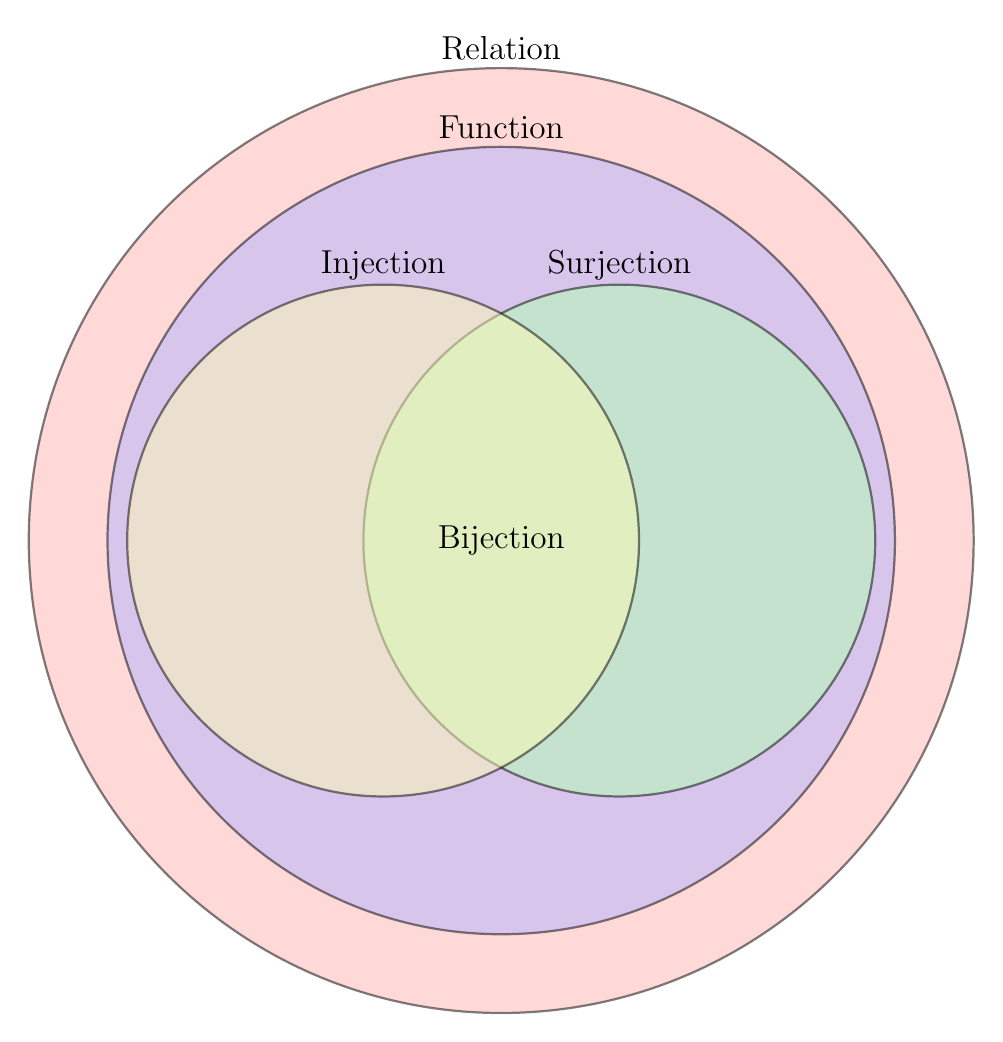
\begin{tikzpicture}
% Define circles
\draw[thick, fill=red!30, opacity=0.5] (0,0) circle (6cm); \node at (0, 6.25) {\large Relation};
\draw[thick, fill=blue!30, opacity=0.5] (0,0) circle (5cm); \node at (0, 5.25) {\large Function};
\draw[thick, fill=green!30, opacity=0.5] (1.5,0) circle (3.25cm); \node at (1.5, 3.5) {\large Surjection};
\draw[thick, fill=yellow!30, opacity=0.5] (-1.5,0) circle (3.25cm); \node at (-1.5, 3.5) {\large Injection};
%\draw[thick, fill=violet!30, opacity=0.5] (0,0) circle (1cm); 
\node at (0, 0) {\large Bijection};
\end{tikzpicture}}
\end{center}
\end{observation}

\section{Functions}
\defbox[Function]{
\begin{definition}
	Let $S$ and $T$ be sets. A \textbf{function} $f$ \textbf{from $\boldmath{S}$ to $\boldmath{T}$} is a relation on $S\times T$ satisfying as follows: \begin{enumerate}[(i)]
		\item (\textbf{Left-Total}\footnote{Every element of $S$ relates to some element of $T$.}) $\dom f=S$, \ie, \[
		s\in S\implies \exists t\in T:f(s)=t.
		\]
		\item (\textbf{Many-to-one}\footnote{Every element of $\dom{f}$ relates to no more than one element of its $\cdm{f}$.}) Let $s\in\dom{f}$ and $t_1,t_2\in\cdm{f}$. Then \[
		f(s)=t_1\land f(s)=t_2\implies s_1=s_2.
		\]
	\end{enumerate}
\end{definition}
}

\defbox[Domain, Codomain, and Range]{
\begin{definition}
\ \begin{itemize}
	\item \textbf{Domain:} The domain of a function \( f: A \to B \) is the set \( A \) of all possible input values for which the function is defined. Formally:
	\[
	\text{Domain}(f) = A
	\]
	\item \textbf{Co-domain:} The co-domain of a function \( f: A \to B \) is the set \( B \) which includes all potential output values. It is the target set for the function. Formally:
	\[
	\text{Co-domain}(f) = B
	\]
	\item \textbf{Range:} The range (or image) of a function \( f \) is the set of all actual output values produced by the function. It is a subset of the co-domain \( B \). Formally:
	\[
	\text{Range}(f) = f[A] = \{ f(a) \mid a \in A \} \subseteq B
	\]
\end{itemize}
\end{definition}
}
\begin{remark}
\ \\ \adjustbox{scale=.9, center}{
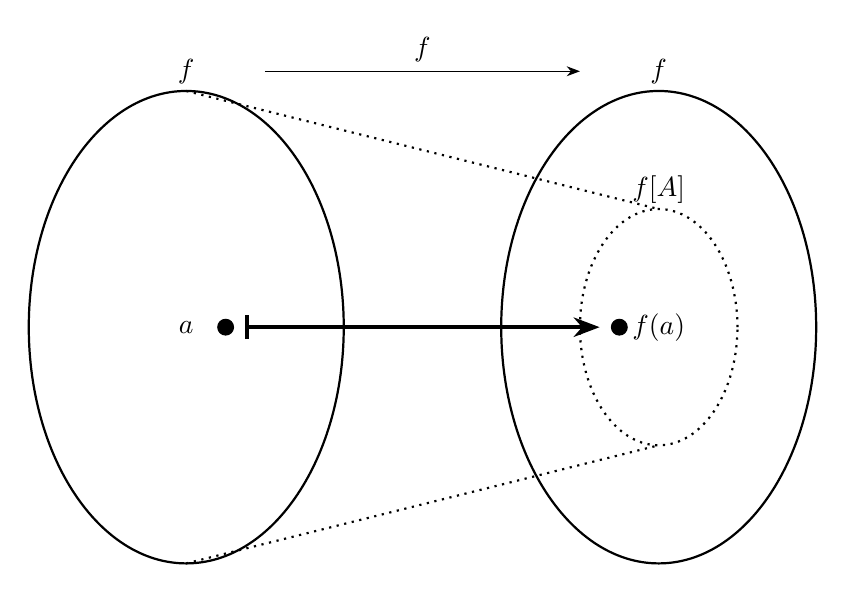
\begin{tikzpicture}
	% Draw the sets A and B
	\draw[thick] (-3,0) ellipse (2 and 3);
	\draw[thick] (3,0) ellipse (2 and 3);
	
	% Labels for sets
	\node at (-3, 3.25) {$\dom f$};
	\node at (3, 3.25) {$\cdm f$};
	
	% Draw the arrows representing the function
	\draw[-Stealth] (-2, 3.25) -- (2,3.25) node[midway, above] {$f$};
	\draw[thick, dotted] (-3,3) -- (3,1.5);
	\draw[thick, dotted] (-3,-3) -- (3,-1.5);
	
	\draw[fill] (-2.5,0) circle (.1);
	\draw[fill] (2.5,0) circle (.1);
	\draw[|-Stealth, line width=.5mm] (-2.25, 0) -- (2.25, 0);
	
	% Labels for elements in Domain
	\node at (-3, 0) {$a$};
	
	% Labels for elements in Co-domain
	\node at (3, 0) {$f(a)$};
	
	% Highlight the range
	\draw[thick, dotted] (3, 0) ellipse (1 and 1.5);
	
	% Label for the range
	\node at (3, 1.75) {$f[A]$};
\end{tikzpicture}}
\end{remark}

\section{Composition}
\defbox[Composition of Functions]{
\begin{definition}
Given two functions \( f \) and \( g \), where \( f: A \to B \) and \( g: B \to C \), the \textbf{composition} of \( g \) and \( f \), denoted by \( g \circ f \), is a function from \( A \) to \( C \) defined as follows:
\[
(g \circ f)(x) = g(f(x))
\]
for all \( x \in A \). That is, \[
\fullfunction{g\circ f}{A}{C}{a}{(g\circ f)(a)}
\]
\end{definition}}
\begin{remark}
\ \begin{itemize}
	\item \textbf{Functions}:
	\begin{itemize}
		\item Let \( f: B \to C \) be a function from set \( B \) to set \( C \).
		\item Let \( g: A \to B \) be a function from set \( A \) to set \( B \).
	\end{itemize}
	
	\item \textbf{Composition Definition}:
	\begin{itemize}
		\item The composition \( f \circ g \) is a function from \( A \) to \( C \).
		\item For each \( x \in A \), \( (f \circ g)(x) \) is defined as \( f(g(x)) \).
	\end{itemize}
	
	\item \textbf{Domain and Range}:
	\begin{itemize}
		\item The domain of the composite function \( f \circ g \) is \( A \).
		\item The range of the composite function \( f \circ g \) is a subset of \( C \).
	\end{itemize}
\end{itemize}
\end{remark}
\vspace{12pt}
\begin{remark}
Let \( G \) be a set of bijective functions from a set \( X \) to itself. Define the binary operation \(\circ\) to be the composition of functions. Then \( G \) under this operation is a group.
\begin{enumerate}
	\item \textbf{Closure}: If \( f, g \in G \), then \( f \circ g \in G \) because the composition of two bijective functions is bijective.
	
	\item \textbf{Associativity}: Function composition is associative. For any \( f, g, h \in G \),
	\[
	(f \circ g) \circ h = f \circ (g \circ h)
	\]
	\adjustbox{scale=.9, center}{
		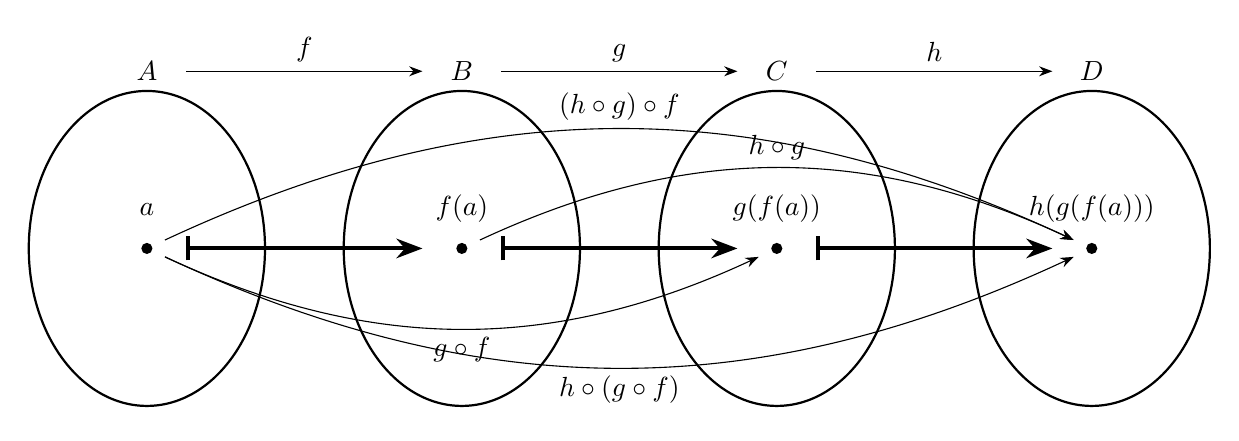
\begin{tikzpicture}
			% Draw the sets A and B
			\draw[thick] (-6,0) ellipse (1.5 and 2);
			\draw[thick] (-2,0) ellipse (1.5 and 2);
			\draw[thick] (2,0) ellipse (1.5 and 2);
			\draw[thick] (6,0) ellipse (1.5 and 2);
			
			% Labels for sets
			\node at (-6, 2.25) {$A$};
			\node at (-2, 2.25) {$B$};
			\node at (2, 2.25) {$C$};
			\node at (6, 2.25) {$D$};
			
			% Draw the arrows representing the function
			\draw[-Stealth] (-5.5, 2.25) -- (-2.5, 2.25) node[midway, above] {$f$};
			\draw[-Stealth] (-1.5, 2.25) -- (1.5, 2.25) node[midway, above] {$g$};
			\draw[-Stealth] (2.5, 2.25) -- (5.5, 2.25) node[midway, above] {$h$};
			\draw[|-Stealth, line width=.5mm] (-5.5, 0) -- (-2.5, 0);
			\draw[|-Stealth, line width=.5mm] (-1.5, 0) -- (1.5, 0);
			\draw[|-Stealth, line width=.5mm] (2.5, 0) -- (5.5, 0);
			
			% Labels for elements in Domain
			\node[fill, circle, inner sep=0.05cm] at (-6,0) (A) {};
			\node[fill, circle, inner sep=0.05cm] at (-2,0) (B) {};
			\node[fill, circle, inner sep=0.05cm] at (2,0) (C) {};
			\node[fill, circle, inner sep=0.05cm] at (6,0) (D) {};
			\node (A2) at (-6, 0.5) {$a$};
			\node (B2) at (-2, 0.5) {$f(a)$};
			\node (C2) at (2, 0.5) {$g(f(a))$};
			\node (D2) at (6, 0.5) {$h(g(f(a)))$};
			
			\draw[-Stealth, bend right=25pt, shorten <= 5pt, shorten >= 5pt] (A) to node[midway,below] {$g\circ f$} (C);
			\draw[-Stealth, bend right=25pt, shorten <= 5pt, shorten >= 5pt] (A) to node[midway,below] {$h\circ(g\circ f)$} (D);
			
			\draw[-Stealth, bend left=25pt, shorten <= 5pt, shorten >= 5pt] (A) to node[midway,above] {$(h\circ g)\circ f$} (D);
			\draw[-Stealth, bend left=25pt, shorten <= 5pt, shorten >= 5pt] (B) to node[midway,above] {$h\circ g$} (D);
	\end{tikzpicture}}
	\item \textbf{Identity Element}: The identity function \( \text{id}_A: A \to A \), defined by \( \text{id}_A(a) = a \) for all \( a \in A \), is the identity element in \( G \). For any \( f \in G \),
	\[
	f \circ \text{id}_A = f = \text{id}_A \circ f
	\]
	\begin{itemize}
		\item[] $f\circ \id_A:$
		\item[] $\id_A\circ f:$
		\item[] $f:$
	\end{itemize}
	\item \textbf{Inverse Element}: For each \( f \in G \), its inverse \( f^{-1} \) exists and is also a bijection from \( A \) to \( A \). It satisfies
	\[
	f \circ f^{-1} = \text{id}_A = f^{-1} \circ f
	\]
\end{enumerate}
\end{remark}

\section{Symmetric Group}
\begin{exercise}[Symmetric Group $S_2$]
The \textbf{symmetric group} \( S_2 \) is the group of all permutations of a two-element set. For a set \( X = \{1, 2\} \), the symmetric group \( S_2 \) consists of all bijective functions (permutations) from \( X \) to itself.

There are exactly two permutations of the set \( S = \{1, 2\} \):
\begin{itemize}
	\item \textbf{Identity Permutation} \( \text{id} \):
	\[
	\text{id}(1) = 1, \quad \text{id}(2) = 2
	\]
	This permutation leaves every element in its original position.\\
	\ \\
	\adjustbox{scale=.9, center}{
		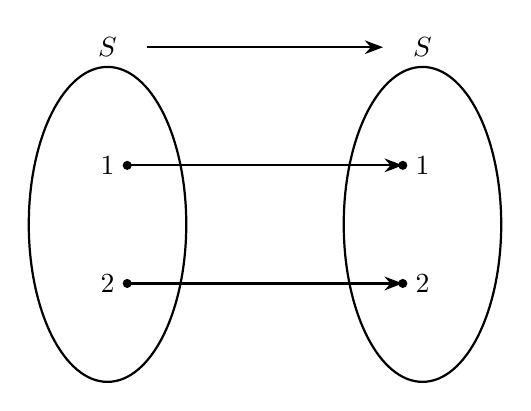
\begin{tikzpicture}
			% Draw the sets A and B
			\draw[thick] (-2,0) ellipse (1 and 2);
			\draw[thick] (2,0) ellipse (1 and 2);
			
			% Labels for sets
			\node at (-2, 2.25) {$S$};
			\node at (2, 2.25) {$S$};
			
%			% Draw the arrows representing the function
			\draw[-Stealth, thick] (-1.5, 2.25) -- (1.5,2.25) node[midway, above] {$\id$};
			
			\node (A) at (-2, .75) {$1$};
			\node (B) at (-2, -.75) {$2$};
			\draw[fill] (-1.75,.75) circle (.05);
			\draw[fill] (-1.75,-.75) circle (.05);
			
			\node (C) at (2, .75) {$1$};
			\node (D) at (2, -.75) {$2$};
			\draw[fill] (1.75,.75) circle (.05);
			\draw[fill] (1.75,-.75) circle (.05);
			
			\draw[-Stealth, thick] (-1.75, .75) -- (1.75, .75);
			\draw[-Stealth, thick] (-1.75, -.75) -- (1.75, -.75);
	\end{tikzpicture}}
	\item \textbf{Transposition} \( \sigma \):
	\[
	\sigma(1) = 2, \quad \sigma(2) = 1
	\]
	This permutation swaps the two elements.\\
	\ \\
	\adjustbox{scale=.9, center}{
		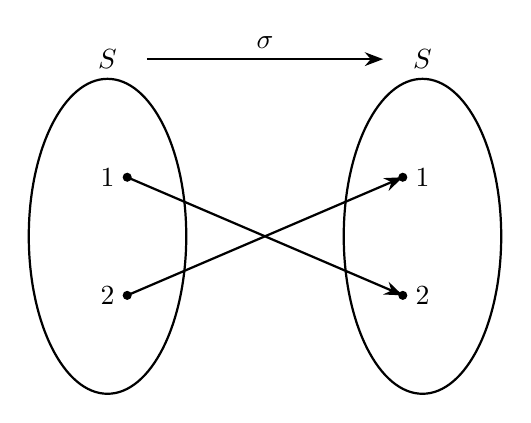
\begin{tikzpicture}
			% Draw the sets A and B
			\draw[thick] (-2,0) ellipse (1 and 2);
			\draw[thick] (2,0) ellipse (1 and 2);
			
			% Labels for sets
			\node at (-2, 2.25) {$S$};
			\node at (2, 2.25) {$S$};
			
			% Draw the arrows representing the function
			\draw[-Stealth, thick] (-1.5, 2.25) -- (1.5,2.25) node[midway, above] {$\sigma$};
			
			\node (A) at (-2, .75) {$1$};
			\node (B) at (-2, -.75) {$2$};
			\draw[fill] (-1.75,.75) circle (.05);
			\draw[fill] (-1.75,-.75) circle (.05);
			
			\node (C) at (2, .75) {$1$};
			\node (D) at (2, -.75) {$2$};
			\draw[fill] (1.75,.75) circle (.05);
			\draw[fill] (1.75,-.75) circle (.05);
			
			\draw[-Stealth, thick] (-1.75, .75) -- (1.75, -.75);
			\draw[-Stealth, thick] (-1.75, -.75) -- (1.75, .75);
	\end{tikzpicture}}
\end{itemize}

Therefore, the elements of \( S_2 \) can be written as:
\[
S_2 = \{ \text{id}, \sigma \}
\]

\end{exercise}
\vspace{12pt}
\begin{exercise}[Symmetric Group $S_3$]
	content...
\end{exercise}

\subsection*{Group Operation}

The group operation in \( S_2 \) is the composition of permutations. Given two permutations \( f \) and \( g \), their composition \( f \circ g \) is defined as:
\[
(f \circ g)(x) = f(g(x))
\]
for all \( x \in X \).

\subsection*{Group Table (Cayley Table)}

The Cayley table for \( S_2 \) describes the result of composing any two permutations:
\[
\begin{array}{c|cc}
	\circ & \text{id} & \sigma \\
	\hline
	\text{id} & \text{id} & \sigma \\
	\sigma & \sigma & \text{id} \\
\end{array}
\]

\subsection*{Group Axioms Verification}

\begin{itemize}
	\item \textbf{Closure}:
	\begin{itemize}
		\item The composition of any two elements in \( S_2 \) is also an element of \( S_2 \).
	\end{itemize}
	
	\item \textbf{Associativity}:
	\begin{itemize}
		\item Function composition is associative. For all \( f, g, h \in S_2 \),
		\[
		(f \circ g) \circ h = f \circ (g \circ h)
		\]
	\end{itemize}
	
	\item \textbf{Identity Element}:
	\begin{itemize}
		\item The identity permutation \(\text{id}\) acts as the identity element. For all \( f \in S_2 \),
		\[
		f \circ \text{id} = \text{id} \circ f = f
		\]
	\end{itemize}
	
	\item \textbf{Inverse Element}:
	\begin{itemize}
		\item Each element in \( S_2 \) has an inverse in \( S_2 \). Specifically,
		\[
		\text{id}^{-1} = \text{id}, \quad \sigma^{-1} = \sigma
		\]
	\end{itemize}
\end{itemize}
%	
%	\newpage
%	\chapter{Group Homomorphism}
%	% Group Homomorphism
\section{Exponentiation Function}

Consider the following groups:
\begin{itemize}
	\item The \textbf{additive group on integers} \((\mathbb{Z}, +)\):
	\begin{itemize}
		\item Set: \(\mathbb{Z}\)
		\item Operation: Addition (+)
		\item Identity Element: 0
		\item Inverses: For each \(a \in \mathbb{Z}\), the inverse is \(-a\).
	\end{itemize}
	
	\item The \textbf{multiplicative group on nonzero rational numbers} \((\mathbb{Q}^*, \cdot)\):
	\begin{itemize}
		\item Set: \(\mathbb{Q}^*\)
		\item Operation: Multiplication (\(\cdot\))
		\item Identity Element: 1
		\item Inverses: For each \(q \in \mathbb{Q}^*\), the inverse is \(q^{-1} = \frac{1}{q}\).
	\end{itemize}
\end{itemize}

We define the exponential function \( \exp : \mathbb{Z} \to \mathbb{Q}^* \) by:
\[
\exp(n) = 2^n \quad \text{for all} \ n \in \mathbb{Z}.
\]

\subsection*{Verification}

\paragraph{Homomorphism Property:}
\[
\exp(a + b) = 2^{a + b} = 2^a \cdot 2^b = \exp(a) \cdot \exp(b).
\]

\paragraph{Identity Element:}
\begin{itemize}
	\item In \((\mathbb{Z}, +)\), the identity element is 0.
	\item In \((\mathbb{Q}^*, \cdot)\), the identity element is 1.
\end{itemize}
\[
\exp(0) = 2^0 = 1.
\]

\paragraph{Inverses:}
\begin{itemize}
	\item For each \( n \in \mathbb{Z} \), the inverse of \( n \) in \(\mathbb{Z}\) is \(-n\).
	\item The inverse of \( \exp(n) = 2^n \) in \(\mathbb{Q}^*\) should be \( \exp(-n) = 2^{-n} \).
\end{itemize}
\[
\exp(-n) = 2^{-n} = \frac{1}{2^n} = (\exp(n))^{-1}.
\]

Thus, the exponential function \( \exp(n) = 2^n \) preserves the group structure between the additive group on integers \((\mathbb{Z}, +)\) and the multiplicative group on nonzero rational numbers \((\mathbb{Q}^*, \cdot)\).

\end{document}
%	
%	\newpage
%	\chapter{Linear Algebra and Group}
%	% Linear Algebra and Group
\begin{note}[General Definition of Vector Space]
The operations $+$ and $\cdot$ must satisfy the following properties for all $\mathbf{u}, \mathbf{v} \in V$ and $\alpha, \beta \in \mathbb{F}$:
\begin{enumerate}
	\item \textbf{Associativity of Addition}:
	\begin{equation*}
		(\mathbf{u} + \mathbf{v}) + \mathbf{w} = \mathbf{u} + (\mathbf{v} + \mathbf{w})
	\end{equation*}
	\item \textbf{Commutativity of Addition}:
	\begin{equation*}
		\mathbf{u} + \mathbf{v} = \mathbf{v} + \mathbf{u}
	\end{equation*}
	\item \textbf{Existence of Additive Identity}:
	\begin{equation*}
		\vec{u}\in V\implies\exists \mathbf{0} \in V:\mathbf{u} + \mathbf{0} = \mathbf{u}
	\end{equation*}
	\item \textbf{Existence of Additive Inverse}:
	\begin{equation*}
		\vec{u}\in V\implies \exists -\mathbf{u} \in V : \mathbf{u} + (-\mathbf{u}) = \mathbf{0}
	\end{equation*}
	\item \textbf{Distributivity of Scalar Multiplication over Vector Addition}:
	\begin{equation*}
		\alpha \cdot (\mathbf{u} + \mathbf{v}) = (\alpha \cdot \mathbf{u}) + (\alpha \cdot \mathbf{v})
	\end{equation*}
	\item \textbf{Distributivity of Scalar Multiplication over Field Addition}:
	\begin{equation*}
		(\alpha + \beta) \cdot \mathbf{u} = (\alpha \cdot \mathbf{u}) + (\beta \cdot \mathbf{u})
	\end{equation*}
	\item \textbf{Compatibility of Scalar Multiplication with Field Multiplication}:
	\begin{equation*}
		(\alpha \beta) \cdot \mathbf{u} = \alpha \cdot (\beta \cdot \mathbf{u})
	\end{equation*}
	\item \textbf{Identity Element of Scalar Multiplication}:
	\begin{equation*}
		1 \cdot \mathbf{u} = \mathbf{u}
	\end{equation*}
\end{enumerate}
\end{note}

\defbox[Linear Operation]{\begin{definition}
Let $V$ be a set over a field $\mathbb{F}$. We define the following linear operations on $V$:
\begin{enumerate}
	\item An \textbf{addition operation} 
	\begin{align*}
		+ : V \times V &\rightarrow V \\
		(\mathbf{u}, \mathbf{v}) &\mapsto \mathbf{u} + \mathbf{v}
	\end{align*}
	on $V$ such that $(V, +)$ is an abelian group.
		
	\item A \textbf{scalar multiplication operation} 
	\begin{align*}
		\cdot : \mathbb{F} \times V &\rightarrow V \\
		(\alpha, \mathbf{u}) &\mapsto \alpha \cdot \mathbf{u}
	\end{align*}
	on $V$. Here $0\cdot\vec{u}:=\vec{0}$ and $1\cdot\vec{u}:=\vec{u}$, \ie, \begin{align*}
		\cdot : \F \times V &\rightarrow V & \cdot : \F \times V &\rightarrow V \\
		(0, \mathbf{u}) &\mapsto \mathbf{0} & (1, \mathbf{u}) &\mapsto \mathbf{u}
	\end{align*}
\end{enumerate}
\end{definition}}
\begin{remark}
Consider \[
\cdot:\F\to[V\to V].
\] Then 
\begin{center}\adjustbox{scale=.9}{
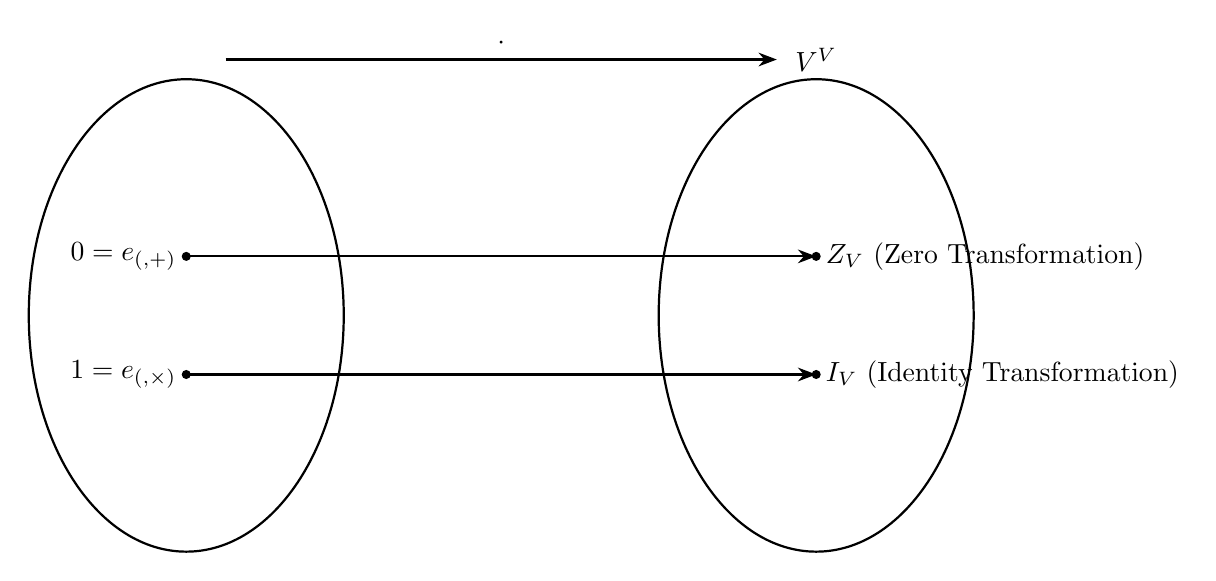
\begin{tikzpicture}
	% Draw the sets A and B
	\draw[thick] (-4,0) ellipse (2 and 3);
	\draw[thick] ( 4,0) ellipse (2 and 3);
	
	% Labels for sets
	\node at (-4, 3.25) {$\F$};
	\node at ( 4, 3.25) {$V^V$};
	
	% Draw the arrows representing the function
	\draw[-Stealth, thick] (-3.5, 3.25) -- (3.5,3.25) node[midway, above] {$\cdot$};
	\draw[fill] (-4,.75) circle (.05) node[left] {$0=e_{(\F,+)}$};
	\draw[fill] (-4,-.75) circle (.05) node[left] {$1=e_{(\F,\times)}$};
	
	\draw[fill] (4,.75) circle (.05) node[right] {$Z_V$ (Zero Transformation)};
	\draw[fill] (4,-.75) circle (.05) node[right] {$I_V$ (Identity Transformation)};
	
	\draw[-Stealth, thick] (-4, .75) -- (4, .75);
	\draw[-Stealth, thick] (-4, -.75) -- (4, -.75);
\end{tikzpicture}}
\end{center}
\end{remark}
\begin{remark}
	Let $V$ be a set over a field $\F$. Assume that, for $\vec{x},\vec{y}\in V$ and $\alpha,\beta\in F$, \[
	\alpha\cdot\vec{x} + \beta\cdot\vec{y}\in V.
	\] Then \[\begin{array}{rcll}
		\alpha=1=\beta &\implies &\vec{x} + \vec{y} \in V &\cdots\cdots\text{(Additivity)} \\
		\beta=0 &\implies &\alpha\cdot \vec{x} \in V &\cdots\cdots\text{(Homogeneity)}
	\end{array}
	\]
\end{remark}

\defbox[Vector Space]{\begin{definition}
A \textbf{vector space} \((V,+,\cdot)\), simply \( V \), over a field \( F \) is a set \( V \) together with two operations:
\begin{enumerate}
	\item \textbf{Vector Addition:} \[
	\fullfunction{+}{V\times V}{V}{(\vec{u},\vec{v})}{\vec{u}+\vec{v}},
	\] such that \( (V, +) \) forms an \underline{abelian group}.
	\item \textbf{Scalar Multiplication:} \[
	\fullfunction{\cdot}{F\times V}{V}{(a,\vec{u})}{a\cdot\vec{u}},
	\] such that \( (V, \cdot) \) satisfies the following properties:
	\begin{enumerate}
		\item \textbf{Distributivity of Scalar Multiplication with Respect to Vector Addition:} \[
		a \cdot (\mathbf{u} + \mathbf{v}) = (a \cdot \mathbf{u}) + (a \cdot \mathbf{v}).
		\]
		\item \textbf{Distributivity of Scalar Multiplication with Respect to Field Addition:} \[
		(a + b) \cdot \mathbf{v} = (a \cdot \mathbf{v}) + (b \cdot \mathbf{v}).
		\]
		\item \textbf{Associativity of Scalar Multiplication:} \[
		a \cdot (b \cdot \mathbf{v}) = (a \cdot b) \cdot \mathbf{v}.
		\]
		\item \textbf{Multiplicative Identity:} \[
		\vec{v}\in V\implies 1 \cdot \mathbf{v} = \mathbf{v},
		\] where 1 is the multiplicative identity in \( F \).
	\end{enumerate}
\end{enumerate}
\end{definition}}

\defbox[Linear Transformation]{\begin{definition}
Let \( V \) and \( W \) be vector spaces over the same field \( F \). A function \( T : V \to W \) is called a \textbf{linear transformation} (or linear map) if for all \( \mathbf{u}, \mathbf{v} \in V \) and all scalars \( a \in F \), the following two conditions are satisfied:

\begin{enumerate}
	\item \textbf{Additivity:} \[
	T(\mathbf{u} + \mathbf{v}) = T(\mathbf{u}) + T(\mathbf{v}).
	\]
	\item \textbf{Homogeneity of Scalar Multiplication:} \[
	T(a \cdot \mathbf{u}) = a \cdot T(\mathbf{u}).
	\]
\end{enumerate}
That is, \( T \) preserves the operations of vector addition and scalar multiplication.
\end{definition}}
\begin{remark}
	\[\begin{cases}
		\vec{u},\vec{v}\in V\\
		a,b\in F
	\end{cases}\implies
	\fullfunction{T}{V}{W}{a\cdot\vec{u}+b\cdot\vec{v}}{T(a\cdot\vec{u}+b\cdot\vec{v})=a\cdot T(\vec{u})+b\cdot T(\vec{v})}
	\]
\end{remark}
\begin{remark}
Given that \( T : V \to W \) is a linear transformation, the following properties hold:
\begin{enumerate}
	\item \( T(\mathbf{0}_V) = \mathbf{0}_W \), where \( \mathbf{0}_V \) and \( \mathbf{0}_W \) are the zero vectors in \( V \) and \( W \), respectively.
	\item \( T\left(\sum_{i=1}^n a_i \mathbf{u}_i\right) = \sum_{i=1}^n a_i T(\mathbf{u}_i) \) for any finite set of vectors \( \mathbf{u}_1, \mathbf{u}_2, \ldots, \mathbf{u}_n \in V \) and scalars \( a_1, a_2, \ldots, a_n \in F \).
\end{enumerate}
\end{remark}
\begin{remark}
\ \begin{center}
\begin{tikzpicture}[auto, node distance=2cm, thick, >=Stealth]
	% Vector Addition
	\node (O1) at (0,0) {};
	\node (U) at (2,1) {};
	\node (V) at (1,2) {};
	\node (U+V) at ($(U) + (V)$) {};
	
	\node (TO1) at (0,-5) {};
	\node (TU) at (2,-4) {};
	\node (TV) at (1,-3) {};
	\node (TU+TV) at (3,-2) {};
	
	% Vectors for Addition
	\draw[->] (O1.center) -- (U.center) node[midway, below right] {$\mathbf{u}$};
	\draw[->] (O1.center) -- (V.center) node[midway, above left] {$\mathbf{v}$};
	\draw[->, dashed] (U.center) -- (U+V.center) node[midway, above right] {};
	\draw[->, dashed] (V.center) -- (U+V.center) node[midway, below left] {};
	\draw[->, very thick, magenta] (O1.center) -- (U+V.center) node[midway, above] {};
	
	\draw[->] (TO1.center) -- (TU.center) node[midway, below right] {$T(\mathbf{u})$};
	\draw[->] (TO1.center) -- (TV.center) node[midway, above left] {$T(\mathbf{v})$};
	\draw[->, dashed] (TU.center) -- (TU+TV.center) node[midway, above right] {};
	\draw[->, dashed] (TV.center) -- (TU+TV.center) node[midway, below left] {};
	\draw[->, very thick, magenta] (TO1.center) -- (TU+TV.center) node[midway, above] {};
	
	% Points for Addition
	\fill (O1) circle (2pt) node[below left] {$\mathbf{O}$};
	\fill (U) circle (2pt) node[below right] {};
	\fill (V) circle (2pt) node[above left] {};
	\fill (U+V) circle (2pt) node[above right] {\textcolor{magenta}{$\mathbf{u} + \mathbf{v}$}};
	
	\fill (TO1) circle (2pt) node[below left] {$\mathbf{O}$};
	\fill (TU) circle (2pt) node[below right] {};
	\fill (TV) circle (2pt) node[above left] {};
	\fill (TU+TV) circle (2pt) node[above right] {\textcolor{magenta}{$T(\mathbf{u}) + T(\mathbf{v})$}};
	
	% Scalar Multiplication
	\node (O2) at (7,0) {};
	\node (U2) at (9,1) {};
	\node (AU2) at ($(O2)!2!(U2)$) {};
	
	\node (TO2) at (7,-5) {};
	\node (TU2) at (9,-4) {};
	\node (TAU2) at (11,-3) {};
	
	% Vectors for Multiplication
	\draw[->] (O2.center) -- (U2.center) node[midway, below right] {$\mathbf{u}$};
	\draw[->, very thick, magenta] (O2.center) -- (AU2.center) node[midway, above] {};
	
	\draw[->] (TO2.center) -- (TU2.center) node[midway, below right] {$T(\mathbf{u})$};
	\draw[->, very thick, magenta] (TO2.center) -- (TAU2.center) node[midway, above] {};
	
	% Points for Multiplication
	\fill (O2) circle (2pt) node[below left] {$\mathbf{O}$};
	\fill (U2) circle (2pt) node[below right] {};
	\fill (AU2) circle (2pt) node[above] {\textcolor{magenta}{$a \cdot \mathbf{u}$}};
	
	\fill (TO2) circle (2pt) node[below left] {$\mathbf{O}$};
	\fill (TU2) circle (2pt) node[below right] {};
	\fill (TAU2) circle (2pt) node[above] {\textcolor{magenta}{$a \cdot T(\mathbf{u})$}};
	
	% Mapping
	\draw[draw=black] (-1, 3.5) rectangle (6,-.5);
	\draw[draw=black] (-1, -1.25) rectangle (6,-5.75);
	\draw[draw=black] (6.25, 3.5) rectangle (13,-.5);
	\draw[draw=black] (6.25, -1.25) rectangle (13,-5.75);
%	\draw[|-Stealth, thick, shorten <= 10pt, shorten >= 5pt] (3, 3) to node[midway, right] {$T(\vec{u}+\vec{v})$} (3,-2);
%	\draw[|-Stealth, thick, shorten <= 10pt, shorten >= 5pt] (11, 2) to node[midway, right] {$T(a\cdot\vec{u})$} (11,-3);
\end{tikzpicture}
%\vspace{36pt}
%\begin{tikzpicture}[auto, node distance=2cm, thick, >=Stealth]
%	% Vector Addition
%	\node (O1) at (0,0) {};
%	\node (U) at (2,1) {};
%	\node (V) at (1,2) {};
%	\node (U+V) at ($(U) + (V)$) {};
%	
%	% Vectors for Addition
%	\draw[->] (O1.center) -- (U.center) node[midway, below right] {$T(\mathbf{u})$};
%	\draw[->] (O1.center) -- (V.center) node[midway, above left] {$T(\mathbf{v})$};
%	\draw[->, dashed] (U.center) -- (U+V.center) node[midway, above right] {};
%	\draw[->, dashed] (V.center) -- (U+V.center) node[midway, below left] {};
%	\draw[->, very thick, magenta] (O1.center) -- (U+V.center) node[midway, above] {};
%	
%	% Points for Addition
%	\fill (O1) circle (2pt) node[below left] {$\mathbf{O}$};
%	\fill (U) circle (2pt) node[below right] {};
%	\fill (V) circle (2pt) node[above left] {};
%	\fill (U+V) circle (2pt) node[above right] {\textcolor{magenta}{$T(\mathbf{u}) + T(\mathbf{v})$}};
%	
%	% Scalar Multiplication
%	\node (O2) at (7,0) {};
%	\node (U2) at (9,1) {};
%	\node (AU2) at ($(O2)!2!(U2)$) {};
%	
%	% Vectors for Multiplication
%	\draw[->] (O2.center) -- (U2.center) node[midway, below right] {$T(\mathbf{u})$};
%	\draw[->, very thick, magenta] (O2.center) -- (AU2.center) node[midway, above] {};
%	
%	% Points for Multiplication
%	\fill (O2) circle (2pt) node[below left] {$\mathbf{O}$};
%	\fill (U2) circle (2pt) node[below right] {};
%	\fill (AU2) circle (2pt) node[above] {\textcolor{magenta}{$a \cdot T(\mathbf{u})$}};
%\end{tikzpicture}
\end{center}
\end{remark}
\begin{remark}[\bf Dimension]
\ \begin{itemize}
	\item (\textbf{Finite-Dimensional Vector Spaces}) A finite-dimensional vector space \( V \) over a field \( F \) with dimension \( n \) is always isomorphic to \( F^n \).
	\item (\textbf{Basis and Isomorphism}) \begin{itemize}
		\item Let \( \{\mathbf{e}_1, \mathbf{e}_2, \ldots, \mathbf{e}_n\} \) be a basis for \( V \).
		\item Any vector \( \mathbf{v} \in V \) can be uniquely expressed as:
		\[
		\mathbf{v} = a_1 \mathbf{e}_1 + a_2 \mathbf{e}_2 + \cdots + a_n \mathbf{e}_n,
		\]
		where \( a_i \in F \) for \( i = 1, 2, \ldots, n \).
		\item The map:
		\[
		\varphi : V \to F^n, \quad \mathbf{v} \mapsto (a_1, a_2, \ldots, a_n)
		\]
		is a linear isomorphism.
	\end{itemize}
	\item (\textbf{Infinite-Dimensional Vector Spaces}) Infinite-dimensional vector spaces are more complex and are not isomorphic to \( F^n \) for any finite \( n \).
	\item (\textbf{Examples and Considerations}) \begin{itemize}
		\item \textbf{Function Spaces}: Spaces like the set of all polynomials \( \mathbb{P} \) or the space of continuous functions \( C([0, 1]) \).
		\item \textbf{Hilbert Spaces}: Spaces such as \( \ell^2 \) (space of square-summable sequences).
		\item \textbf{Isomorphisms}: Infinite-dimensional vector spaces may be isomorphic to structures like \( F^\infty \) (sequences with only finitely many non-zero entries) or \( F^{(\infty)} \) (the direct sum of infinitely many copies of \( F \)).
	\end{itemize}
\end{itemize}
\end{remark}


%	
%	From the standpoint of solving equations, the algebraic structures we have discussed are interconnected in the following ways:
%	
%	\subsection*{Group}
%	A \textbf{group} provides a foundation for solving equations involving a single operation. The group structure ensures that every element has an inverse, allowing us to "undo" operations and solve equations. For instance, in the group of integers \( (\mathbb{Z}, +) \), the equation \( x + a = b \) can be solved as \( x = b - a \).
%	
%	\subsection*{Ring}
%	A \textbf{ring} extends the concept of a group by introducing a second operation, typically multiplication, in addition to addition. Rings allow us to solve more complex equations that involve both addition and multiplication. For example, solving polynomial equations \( f(x) = 0 \) where \( f(x) \) is a polynomial with coefficients in a ring \( R \).
%	
%	\subsection*{Field}
%	A \textbf{field} is a ring with additional properties that make division possible (except by zero). This structure is crucial for solving linear equations and systems of linear equations. In a field \( F \), any linear equation \( ax = b \) (where \( a \neq 0 \)) can be solved as \( x = a^{-1}b \), where \( a^{-1} \) is the multiplicative inverse of \( a \).
%	
%	\subsection*{Vector Space}
%	A \textbf{vector space} over a field \( F \) is a set of vectors that can be added together and scaled by elements of \( F \). Vector spaces provide a framework for solving linear systems of equations. Solutions to systems of linear equations can be understood as finding vectors \( \mathbf{x} \in V \) such that \( A\mathbf{x} = \mathbf{b} \), where \( A \) is a matrix and \( \mathbf{b} \) is a vector in \( V \).
%	
%	\subsection*{Module}
%	A \textbf{module} is a generalization of vector spaces where the scalars come from a ring instead of a field. Modules allow us to solve equations in contexts where the coefficients are not from a field, such as systems of linear equations with integer coefficients. For example, solving \( A\mathbf{x} = \mathbf{b} \) where \( A \) is a matrix with entries from a ring \( R \) and \( \mathbf{x}, \mathbf{b} \in M \).
%	
%	\subsection*{Algebra}
%	An \textbf{algebra} over a field \( F \) combines the structures of a vector space and a ring. Algebras provide a framework for solving polynomial equations and other equations involving both addition and multiplication of vectors. In an algebra \( A \), we can solve equations like \( x^2 + ax + b = 0 \) using techniques from both linear algebra and ring theory.
%	
%	\subsection*{Summary}
%	The conceptual connection between these structures is rooted in the increasing complexity and capability they offer for solving equations:
%	\begin{itemize}
%		\item \textbf{Groups} provide a way to solve equations with a single operation.
%		\item \textbf{Rings} introduce a second operation, allowing for more complex equations.
%		\item \textbf{Fields} enable division, which is essential for solving linear equations.
%		\item \textbf{Vector spaces} over fields extend these concepts to systems of linear equations.
%		\item \textbf{Modules} generalize vector spaces to allow coefficients from rings.
%		\item \textbf{Algebras} integrate vector space and ring structures, enabling the solution of polynomial and other complex equations.
%	\end{itemize}
%	
%	\newpage
%	\chapter*{LaTex Practice}
%	\begin{itemize}
	\item \textbf{Block Size}: $n$ (number of bits in a block)
	\item \textbf{Key Size}: $k$ (number of bits in the key)
\end{itemize}
\begin{align*}
	E:\boxed{\set{0,1}^k\times\set{0,1}^n}\to\set{0,1}^n \\
	D:\boxed{\set{0,1}^k\times\set{0,1}^n}\to\set{0,1}^n
\end{align*}
\adjustbox{scale=.9, center}{
	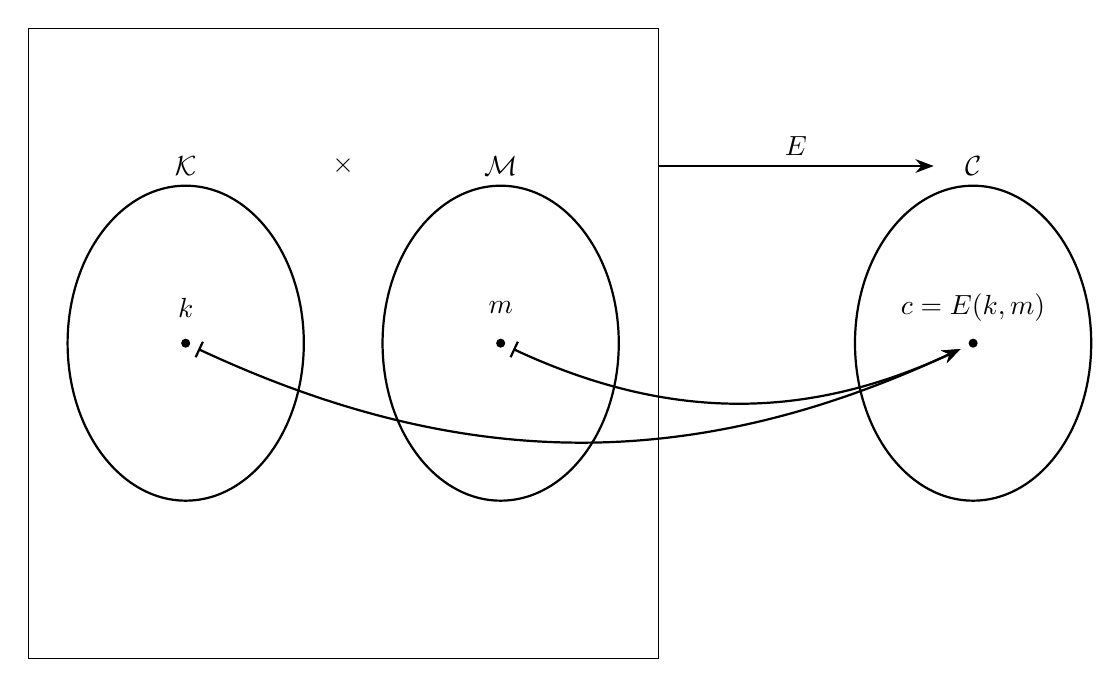
\begin{tikzpicture}
		% Draw the sets A and B
		\draw[thick] (-6,0) ellipse (1.5 and 2);
		\draw[thick] (-2,0) ellipse (1.5 and 2);
		\draw[thick] (4,0) ellipse (1.5 and 2);
		\draw[draw=black] (-8, 4) rectangle (0,-4);
		% Labels for sets
		\node at (-6, 2.25) {$\mathcal{K}$};
		\node at (-4, 2.25) {$\times$};
		\node at (-2, 2.25) {$\mathcal{M}$};
		\node at (4, 2.25) {$\mathcal{C}$};
		
		% Draw the arrows representing the function
		\draw[-Stealth, thick] (0, 2.25) -- (3.5,2.25) node[midway, above] {$E$};
		
		\node (K) at (-6, .45) {$k$};
		\node (M) at (-2, .45) {$m$};
		\node (C) at (4, .45) {$c=E(k,m)$};
		\draw[fill] (-6,0) circle (.05);
		\draw[fill] (-2,0) circle (.05);
		\draw[fill] (4,0) circle (.05);
		
		\draw[|-Stealth, thick, bend right=25pt, shorten <= 5pt, shorten >= 5pt] (-6, 0) to node[midway,below] {} (4,0);
		\draw[|-Stealth, thick, bend right=25pt, shorten <= 5pt, shorten >= 5pt] (-2, 0) to node[midway,below] {} (4,0);
\end{tikzpicture}}
\begin{align*}
	E:\set{0,1}^k\to\boxed{\set{0,1}^n\to\set{0,1}^n} \\
	D:\set{0,1}^k\to\boxed{\set{0,1}^n\to\set{0,1}^n}
\end{align*}
\adjustbox{scale=.9, center}{
	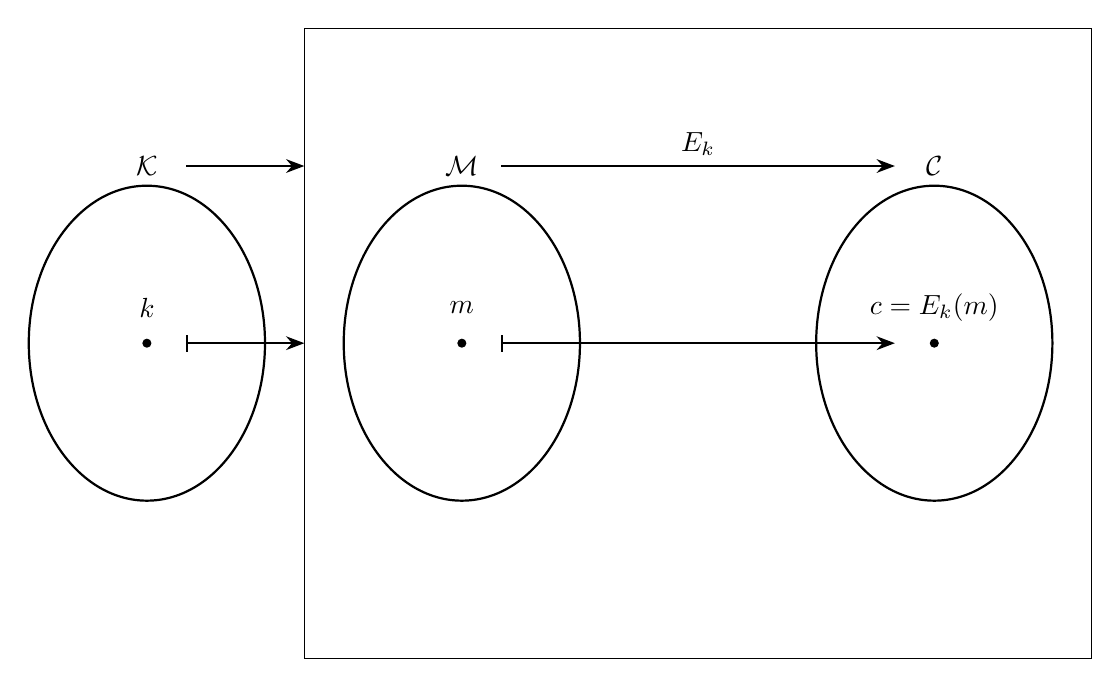
\begin{tikzpicture}
		% Draw the sets A and B
		\draw[thick] (-6,0) ellipse (1.5 and 2);
		\draw[thick] (-2,0) ellipse (1.5 and 2);
		\draw[thick] (4,0) ellipse (1.5 and 2);
		\draw[draw=black] (-4, 4) rectangle (6,-4);
		% Labels for sets
		\node at (-6, 2.25) {$\mathcal{K}$};
		\node at (-2, 2.25) {$\mathcal{M}$};
		\node at (4, 2.25) {$\mathcal{C}$};
		
		% Draw the arrows representing the function
		\draw[-Stealth, thick] (-1.5, 2.25) -- (3.5,2.25) node[midway, above] {$E_k$};
		\draw[-Stealth, thick] (-5.5, 2.25) -- (-4,2.25) node[midway, above] {};
		
		\node (K) at (-6, .45) {$k$};
		\node (M) at (-2, .45) {$m$};
		\node (C) at (4, .45) {$c=E_k(m)$};
		\draw[fill] (-6,0) circle (.05);
		\draw[fill] (-2,0) circle (.05);
		\draw[fill] (4,0) circle (.05);
		
		\draw[|-Stealth, thick] (-5.5, 0) to node[midway,below] {} (-4,0);
		\draw[|-Stealth, thick] (-1.5, 0) to node[midway,below] {} (3.5,0);
\end{tikzpicture}}
%	
%	% Appendix
%	\newpage
%	\appendix
%	\chapter{Preliminaries}
\section{Sets, Cartesian Products, and Relations}

\subsection{Sets and Ordered Pairs}

\subsection*{Set}

A \textbf{set} is a well-defined collection of distinct objects, called elements or members of the set. Sets are one of the most fundamental concepts in mathematics.

\defbox[Set]{
\begin{definition}
	A \textbf{set} is a well-defined collection of distinct objects, considered as an object in its own right. Sets are usually denoted by capital letters, and the elements are listed within curly braces.
\end{definition}
}
\begin{example}
For example:
\[
A = \{1, 2, 3\}
\]
This denotes a set \(A\) containing the elements 1, 2, and 3.
\end{example}
\vspace{12pt}
\begin{note}[Properties]
\ \begin{itemize}
	\item \textbf{No Repetition}: Each element in a set appears only once.
	\item \textbf{Order Irrelevance}: The order of elements in a set does not matter. For instance, \(\{1, 2, 3\} = \{3, 2, 1\}\).
	\item \textbf{Membership}: If an element \(a\) is in a set \(A\), we write \(a \in A\).
\end{itemize}
\end{note}
\vspace{12pt}
\begin{note}[Types of Sets]
\ \begin{itemize}
	\item \textbf{Finite and Infinite Sets}: A set with a finite number of elements is finite; otherwise, it is infinite.
	\item \textbf{Subset}: A set \(A\) is a subset of a set \(B\) if every element of \(A\) is also an element of \(B\), denoted \(A \subseteq B\).
	\item \textbf{Power Set}: The power set of \(A\) is the set of all subsets of \(A\), denoted \(\mathcal{P}(A)\).
\end{itemize}
\end{note}

\subsection*{Ordered Pair}

An \textbf{ordered pair} is a fundamental concept in mathematics used to combine two elements in a specific order. The notation for an ordered pair is \((a, b)\), where \(a\) is the first element and \(b\) is the second element.

\defbox[Ordered Pair]{
\begin{definition}
	An \textbf{ordered pair} \((a, b)\) is a collection of two elements where the order of the elements matters. This is in contrast to a set, where the order of elements does not matter.
\end{definition}
}
\begin{remark}
	\ \begin{itemize}
		\item The ordered pair \((a, b)\) is not the same as \((b, a)\) unless \(a = b\).
		\item Formally, the ordered pair \((a, b)\) can be defined using sets to ensure the distinction from unordered pairs. One common definition is:
		\[
		(a, b) = \{ \{a\}, \{a, b\} \}
		\]
		This definition ensures that:
		\[
		(a, b) = (c, d) \iff a = c \ \text{and} \ b = d
		\]
	\end{itemize}
\end{remark}
\vspace{12pt}
\begin{note}[Properties]
\begin{itemize}
	\item \textbf{Uniqueness}: Each ordered pair \((a, b)\) is unique if either \(a\) or \(b\) is unique.
	\item \textbf{Order}: The order of elements in an ordered pair is significant.
\end{itemize}
\end{note}

\subsection{Cartesian Product and Relation}

\subsection*{Cartesian Product}

The \textbf{Cartesian product} is a fundamental concept in set theory, used to define the set of all possible ordered pairs from two sets.

\defbox[Cartesian Product]{
Given two sets \( A \) and \( B \), the Cartesian product \( A \times B \) is defined as the set of all ordered pairs \((a, b)\) where \( a \in A \) and \( b \in B \). Formally,
\[
A \times B = \{ (a, b) \mid a \in A \ \text{and} \ b \in B \}
\]
}
\vspace{12pt}
\begin{note}[Properties]
\ \begin{itemize}
	\item \textbf{Order Matters}: The pair \((a, b)\) is different from the pair \((b, a)\) unless \(a = b\).
	\item \textbf{Empty Set}: If either \(A\) or \(B\) is the empty set \(\emptyset\), then \(A \times B\) is also empty:
	\[
	A \times \emptyset = \emptyset \quad \text{and} \quad \emptyset \times B = \emptyset
	\]
\end{itemize}
\end{note}
\begin{example}
\ \begin{enumerate}
	\item If \( A = \{1, 2\} \) and \( B = \{x, y\} \), then
	\[
	A \times B = \{ (1, x), (1, y), (2, x), (2, y) \}
	\]
	
	\item If \( A = \{a, b\} \) and \( B = \{1, 2, 3\} \), then
	\[
	A \times B = \{ (a, 1), (a, 2), (a, 3), (b, 1), (b, 2), (b, 3) \}
	\]
\end{enumerate}
\end{example}

\subsection*{Relation}

A \textbf{relation} generalizes the concept of Cartesian product to establish connections between elements of two sets.

\defbox[Relation]{
\begin{definition}
	A relation \( R \) from a set \( A \) to a set \( B \) is a subset of the Cartesian product \( A \times B \). Formally,
	\[
	R \subseteq A \times B
	\]
	This means that a relation \( R \) consists of ordered pairs \((a, b)\) where \(a \in A\) and \(b \in B\).
\end{definition}
}
\vspace{12pt}
\begin{note}[Properties of Relations]
\ \begin{itemize}
	\item \textbf{Domain and Range}:
	\begin{itemize}
		\item The \textbf{domain} of \( R \) is the set of all \( a \in A \) such that there exists \( b \in B \) with \((a, b) \in R\).
		\[
		\text{Domain}(R) = \{ a \in A \mid \exists b \in B, \ (a, b) \in R \}
		\]
		\item The \textbf{range} of \( R \) is the set of all \( b \in B \) such that there exists \( a \in A \) with \((a, b) \in R\).
		\[
		\text{Range}(R) = \{ b \in B \mid \exists a \in A, \ (a, b) \in R \}
		\]
	\end{itemize}
	
	\item \textbf{Inverse Relation}: The inverse of a relation \( R \), denoted \( R^{-1} \), is the set of all pairs \((b, a)\) such that \((a, b) \in R\):
	\[
	R^{-1} = \{ (b, a) \mid (a, b) \in R \}
	\]
	
	\item \textbf{Composition of Relations}: Given a relation \( R \) from \( A \) to \( B \) and a relation \( S \) from \( B \) to \( C \), the composition \( S \circ R \) is a relation from \( A \) to \( C \) defined by:
	\[
	S \circ R = \{ (a, c) \mid \exists b \in B, \ (a, b) \in R \ \text{and} \ (b, c) \in S \}
	\]
\end{itemize}
\end{note}

\vspace{12pt}
\begin{note}[Types of Relations]
\ \begin{itemize}
	\item \textbf{Binary Relation}: A relation involving two sets, as defined above.
	\item \textbf{Unary Relation}: A relation on a single set \( A \) is simply a subset of \( A \).
	\item \textbf{Ternary and Higher Relations}: Relations involving three or more sets, defined as subsets of the Cartesian product of those sets.
\end{itemize}
\end{note}

\begin{example}
	\ \begin{enumerate}
		\item If \( A = \{1, 2, 3\} \) and \( B = \{a, b\} \), a possible relation \( R \) from \( A \) to \( B \) could be:
		\[
		R = \{ (1, a), (2, b), (3, a) \}
		\]
		\begin{itemize}
			\item Domain: \(\{1, 2, 3\}\)
			\item Range: \(\{a, b\}\)
		\end{itemize}
		
		\item Consider the relation \( R \) on set \( A = \{1, 2, 3\} \) defined by:
		\[
		R = \{ (1, 2), (2, 3), (3, 1) \}
		\]
		\begin{itemize}
			\item Domain: \(\{1, 2, 3\}\)
			\item Range: \(\{1, 2, 3\}\)
			\item Inverse Relation: \( R^{-1} = \{ (2, 1), (3, 2), (1, 3) \} \)
		\end{itemize}
	\end{enumerate}
\end{example}

\section{Rational Number and Equivalence Class}

We define the equivalence relation \((a, b) \sim (c, d)\) on the set \(\mathbb{Z} \times \mathbb{Z}^*\) as:
\[
(a, b) \sim (c, d) \iff ad = bc
\]
\begin{proof}
To prove that \(\sim\) is an equivalence relation, we must show it is reflexive, symmetric, and transitive.
\begin{itemize}
	\item \textbf{Reflexive}: A relation \(\sim\) is reflexive if every element is related to itself.
	
	For any \((a, b) \in \mathbb{Z} \times \mathbb{Z}^*\), we need to show that \((a, b) \sim (a, b)\).
	\[
	(a, b) \sim (a, b) \iff ab = ba
	\]
	This is true because \(ab = ba\) holds for all integers \(a\) and \(b\).
	Thus, the relation is reflexive.
	\item \textbf{Symmetric}: A relation \(\sim\) is symmetric if whenever \((a, b) \sim (c, d)\), then \((c, d) \sim (a, b)\).
	
	Assume \((a, b) \sim (c, d)\). This means:
	\[
	ad = bc
	\]
	We need to show that \((c, d) \sim (a, b)\).
	\[
	(c, d) \sim (a, b) \iff cd = da
	\]
	Since \(ad = bc\), we have \(cd = da\) by the commutative property of multiplication.
	Thus, the relation is symmetric.
	\item \textbf{Transitive}: A relation \(\sim\) is transitive if whenever \((a, b) \sim (c, d)\) and \((c, d) \sim (e, f)\), then \((a, b) \sim (e, f)\).
	
	Assume \((a, b) \sim (c, d)\) and \((c, d) \sim (e, f)\). This means:
	\[
	ad = bc \quad \text{and} \quad cf = de
	\]
	We need to show that \((a, b) \sim (e, f)\).
	\[
	(a, b) \sim (e, f) \iff af = be
	\]
	From \(ad = bc\), we have \(d = \frac{bc}{a}\) (assuming \(a \neq 0\)). Substituting \(d\) into \(cf = de\):
	\[
	c f = \left(\frac{bc}{a}\right) e
	\]
	Multiplying both sides by \(a\):
	\[
	a c f = b c e
	\]
	Since \(c \neq 0\):
	\[
	a f = b e
	\]
	Thus, \((a, b) \sim (e, f)\), proving that the relation is transitive.	
\end{itemize}
\end{proof}

Since the relation \((a, b) \sim (c, d) \iff ad = bc\) is reflexive, symmetric, and transitive, it is an equivalence relation on \(\mathbb{Z} \times \mathbb{Z}^*\).


The equivalence relation \((a, b) \sim (c, d) \iff ad = bc\) naturally connects to the division of the set of pairs of integers into equivalence classes, where each equivalence class represents a unique rational number.

An equivalence class \([(a, b)]\) under this relation consists of all pairs \((c, d)\) such that \((a, b) \sim (c, d)\). This can be interpreted as:
\[
[(a, b)] = \{ (c, d) \mid ad = bc \}
\]

Each equivalence class \([(a, b)]\) corresponds to the rational number \(\frac{a}{b}\), and different pairs \((a, b)\) and \((c, d)\) represent the same rational number if and only if they belong to the same equivalence class.

\begin{example}
Consider \((1, 2)\), \((2, 4)\), \((3, 6)\), \((-1, -2)\), \((1, -2)\)
\begin{itemize}
	\item (Class of $(1,2)$)
\[
[1, 2] = \{ (c, d) \in \mathbb{Z} \times \mathbb{Z}^* \mid 1d = 2c \} = \{ (1, 2), (2, 4), (3, 6), (-1, -2), \ldots \}
\]
This class represents the rational number \(\frac{1}{2}\).
\item (Class of $(2,3)$)
\[
[2, 3] = \{ (c, d) \in \mathbb{Z} \times \mathbb{Z}^* \mid 2d = 3c \} = \{ (2, 3), (4, 6), (-2, -3), \ldots \}
\]
This class represents the rational number \(\frac{2}{3}\).
\item (Class of $(1,-2)$)
\[
[1, -2] = \{ (c, d) \in \mathbb{Z} \times \mathbb{Z}^* \mid 1d = -2c \} = \{ (1, -2), (2, -4), (-1, 2), \ldots \}
\]
This class represents the rational number \(\frac{1}{-2}\).
\end{itemize}
\end{example}

\begin{remark}[Properties of Partition]
\ \begin{itemize}
	\item (Disjoint) Each element of \(\mathbb{Z} \times \mathbb{Z}^*\) belongs to exactly one equivalence class. If \((a, b) \in [c, d]\), then \([a, b] = [c, d]\).
	\item (Exhaustive) The union of all equivalence classes covers the entire set \(\mathbb{Z} \times \mathbb{Z}^*\). Every pair \((a, b) \in \mathbb{Z} \times \mathbb{Z}^*\) is in some equivalence class.
\end{itemize}
\end{remark}

\section*{Bijection Between \(\mathbb{Z} \times \mathbb{Z}^*\) and \(\mathbb{N}\)}

To establish a bijection between \(\mathbb{Z} \times \mathbb{Z}^*\) and \(\mathbb{N}\), we construct a function that maps each pair \((a, b)\) in \(\mathbb{Z} \times \mathbb{Z}^*\) to a unique natural number.

\subsection*{Encoding Integers as Natural Numbers}

Define the encoding function \(e: \mathbb{Z} \to \mathbb{N}\) as follows:
\[
e(a) =
\begin{cases}
	2a & \text{if } a \geq 0 \\
	-2a - 1 & \text{if } a < 0
\end{cases}
\]

Define the encoding function \(e^*: \mathbb{Z}^* \to \mathbb{N}\) similarly:
\[
e^*(b) =
\begin{cases}
	2b & \text{if } b > 0 \\
	-2b - 1 & \text{if } b < 0
\end{cases}
\]

\subsection*{Pairing Function}

Define a pairing function \(\pi: \mathbb{N} \times \mathbb{N} \to \mathbb{N}\) by:
\[
\pi(n_1, n_2) = \frac{(n_1 + n_2)(n_1 + n_2 + 1)}{2} + n_2
\]

\subsection*{Mapping Function}

Define the mapping function \(f: \mathbb{Z} \times \mathbb{Z}^* \to \mathbb{N}\) by:
\[
f(a, b) = \pi(e(a), e^*(b))
\]

\subsection*{Bijection}

To show that \(f\) is a bijection, we need to prove that it is both injective and surjective.

\subsubsection*{Injectivity}

Assume \(f(a, b) = f(c, d)\). This implies:
\[
\pi(e(a), e^*(b)) = \pi(e(c), e^*(d))
\]
Since \(\pi\) is injective, we have:
\[
(e(a), e^*(b)) = (e(c), e^*(d))
\]
This implies \(e(a) = e(c)\) and \(e^*(b) = e^*(d)\), which in turn implies \(a = c\) and \(b = d\).

Thus, \(f\) is injective.

\subsubsection*{Surjectivity}

Let \(n \in \mathbb{N}\). We need to find \((a, b) \in \mathbb{Z} \times \mathbb{Z}^*\) such that \(f(a, b) = n\).

Since \(\pi\) is surjective, there exist \(n_1, n_2 \in \mathbb{N}\) such that:
\[
n = \pi(n_1, n_2)
\]
Using the inverse of \(e\) and \(e^*\), we can find \(a\) and \(b\) such that:
\[
e(a) = n_1 \quad \text{and} \quad e^*(b) = n_2
\]

Thus, \(f(a, b) = n\), and \(f\) is surjective.

\subsection*{Conclusion}

Since \(f\) is both injective and surjective, it is a bijection. Therefore, \(\mathbb{Z} \times \mathbb{Z}^*\) is in one-to-one correspondence with \(\mathbb{N}\).

\section*{Invalid Equivalence Classes and Proof Using Natural Numbers and Integers}

Consider the equivalence relation \((a, b) \sim (c, d)\) defined by:
\[
(a, b) \sim (c, d) \iff ad = bc
\]
where \((a, b), (c, d) \in \mathbb{Z} \times \mathbb{Z}^*\) and \(\mathbb{Z}^* = \mathbb{Z} \setminus \{0\}\).

\subsection*{Invalid Equivalence Classes}

\subsubsection*{Equivalence Classes Overview}

In mathematics, an equivalence class under a given equivalence relation is a subset formed by grouping all elements related to each other by that relation. For the relation \((a, b) \sim (c, d) \iff ad = bc\) on \(\mathbb{Z} \times \mathbb{Z}^*\), each equivalence class represents a unique rational number.

\subsubsection*{Valid Equivalence Classes}

Under the relation \((a, b) \sim (c, d) \iff ad = bc\) with \( b \neq 0 \) and \( d \neq 0 \), each equivalence class \([a, b]\) includes all pairs \((c, d)\) such that \( ad = bc \). Formally:
\[
[a, b] = \{(c, d) \in \mathbb{Z} \times \mathbb{Z}^* \mid ad = bc\}
\]
These equivalence classes correspond to unique relationships between pairs of integers.

\subsubsection*{Invalid Equivalence Classes with Zero Denominator}

When \( b = 0 \) or \( d = 0 \), the equivalence relation breaks down because:

\begin{itemize}
	\item \textbf{Undefined Products}: A pair \((a, 0)\) does not represent a valid mathematical entity since \(a \cdot 0\) is not meaningful in the context of this relation.
	\item \textbf{Equivalence Condition Breakdown}: If \( b = 0 \) or \( d = 0 \), the condition \( ad = bc \) can lead to contradictions or meaningless comparisons.
\end{itemize}

\subsection*{Proof: If \( b = 0 \) or \( d = 0 \), Then \((a, b)\) is Not Equivalent to \((c, d)\)}

\subsubsection*{Case 1: \( b = 0 \) and \( d \neq 0 \)}

Suppose \((a, 0) \sim (c, d)\). According to the equivalence relation:
\[
a \cdot d = 0 \cdot c \implies ad = 0
\]
For this to hold, at least one of \(a\) or \(d\) must be zero. Given that \(d \neq 0\), we must have \(a = 0\). Thus:
\[
(a, 0) \sim (0, d)
\]
This implies that \((a, 0)\) can only be equivalent to pairs of the form \((0, d)\).

\subsubsection*{Case 2: \( d = 0 \) and \( b \neq 0 \)}

Suppose \((a, b) \sim (c, 0)\). According to the equivalence relation:
\[
a \cdot 0 = b \cdot c \implies 0 = bc
\]
For this to hold, at least one of \(b\) or \(c\) must be zero. Given that \(b \neq 0\), we must have \(c = 0\). Thus:
\[
(a, b) \sim (0, 0)
\]
This implies that \((c, 0)\) can only be equivalent to pairs of the form \((a, 0)\).

\subsubsection*{Case 3: Both \( b = 0 \) and \( d = 0 \)}

Suppose \((a, 0) \sim (c, 0)\). According to the equivalence relation:
\[
a \cdot 0 = 0 \cdot c \implies 0 = 0
\]
This is trivially true, so pairs of the form \((a, 0)\) are all equivalent to each other, regardless of the value of \(a\) or \(c\).

\subsection*{Conclusion}

When \( b = 0 \) or \( d = 0 \), the equivalence relation \((a, b) \sim (c, d) \iff ad = bc\) does not define valid equivalence classes that can represent meaningful relationships between pairs of integers. These invalid equivalence classes do not correspond to well-defined mathematical entities because they involve undefined or meaningless products.

	
\end{document}
